\documentclass[12pt, a4paper]{report}   % list options between brackets
\usepackage{setspace}
\usepackage{graphicx}
\usepackage{float}
\usepackage{rotating}
\graphicspath{../content/}



\begin{document}

\begin{center}


% Upper part of the page
\textsc{\large University of Sussex}\\[1.5cm]
\textsc{Final year project}\\[2cm]


% Title
\begin{spacing}{2.5}
{\Large \bfseries Estimating personal energy expenditure \\ with location data}\\[5 cm]
\end{spacing}
\end{center}
\vfill


% Author and supervisor
\begin{spacing}{1.5}
\begin{tabular}{l}
Student Name: Vladimir Hartmann \\
Degree program: BSc Computer Science \\
Department: School of Informatics \\
Candidate Number: 52665 \\
Project Supervisor: Dr. Martin Berger \\
Date of Submission: {\today}
\end{tabular}
\end{spacing}
\thispagestyle{empty}


% Statement of originality
\clearpage
\pagenumbering{roman}
\section*{Statement of Originality}
This report is submitted as part requirement for the degree of Computer Science at the University of Sussex. It is the product of my own labour except where indicated in the text. The report may be freely copied and distributed provided the source is acknowledged.


% Summary
\clearpage
\section*{Summary}


% Table of content
\tableofcontents
\thispagestyle{empty}


% Introduction
\clearpage
\pagenumbering{arabic}
\chapter{Introduction}
Modern society is putting unsustainable demands on personal wellbeing as well as the wellbeing of the planet. Pervasive sedentary lifestyle has been creating many health conditions while excess in energy consumption has had adverse effects on our ecosystem. There is a clear connection between personal and planetary wellbeing and actions that help to improve our own health often have a positive effect on our environment. The aim of this project was to create a personal energy meter (PEM), which would measure caloric expenditure and carbon footprint of individual. Idea behind PEM is to have device that would be capable of providing information about a caloric cost and cost of the carbon dioxide of various activities a person is involved in during the day. By wide distribution of PEM people's awareness could increase which would lead to healthier society and cleaner planet. Location data such as those provided by GPS can be utilised to address both issues. As it is most frequently collected piece of contextual data in computing, it can be applied to many healthcare applications. This technique offers a number of improvements over traditional methods, which involve carrying a dedicated accelerometer device.


% Background
\chapter{Background}
On-going progress is being made by various universities and institutes to address the issue of personal energy expenditure monitoring. This is due to the fact that the global economy is not able to meet the minimum conditions for sustainability. The Rio Declaration of 1992 and the United Nations Millennium Development Goals have demonstrated that human demand for ecosystem goods and services exceed the biosphere's total capacity. A fundamental solution is to manage food, fibre and energy consumption and maintain or increase the productivity of natural and agricultural ecosystems. From the number of proposed solutions, the 'shrink and share' framework has gained increasing recognition. This solution emphasises an equal allocation of emission rights to each person on the Earth and has been established by European Parliament as a basic principle to reducing global emissions of carbon dioxide [2].  Simon Hay at University of Cambridge proposed a 'Global Personal Energy Meter' (PEM) device [1], which can record and apportion an individual's energy usage. Architecture of this PEM would consist of a global sensor network and devices such as smartphones would communicate with it and receive estimates of energy used by individual. Data from a 'world model' (recommended energy usage allocations) would be fed into PEM to estimates keep up-to-date.  Further research undertaken by Simon Hay, this time together with Stamatina Th. Rassia , Dr. Alastair Beresford and Dr. Nick V. Baker include 'Movement dynamics in office environment' [3] and 'Estimating personal energy expenditure with location data' [4]. The task of this research was to explore the relationship between indoor environments and physical activity by gathering location and physical activity data. Devices used in an experiment were Active Bat location tracking device and GTIM Actigraph. To estimate personal energy expenditure an energy consumption model had to calculate gravitational and kinetic energy.

Tracking people's movement has been known for some time now. Romans used odometer calibrated to steps, although technically not a step counter, the idea was similar. Leonardo Da Vinci designed a mechanical pedometer, which was used for civil and military purposes. Most of the movements tracking solution on the market today make use accelerometer, which is a device able to monitor any movement in X, Y and Z coordinates. This approach however requires wearing a special device, which might not me convenient. It is also not accurate in many cases (user can cheat by only moving the device in certain way to mimic the actual walking/running).
Proposed approach in this project uses mainly GPS data to track users movement. This can be supported (with project extensions) by accelerometer data and data obtained from signals of the heartbeat. All three technologies combined can produce very accurate and reliable system.
…. Needs re-write


% Professional Considerations
\chapter{Professional Considerations}
Code of Conduct
The project raises the issue set out in section 1, subsection (a) of Code of Conduct. Implementation of Personal Energy Meter (PEM) requires use of the iPhone Location Services that gather location data of user. It must be assured that any storage or transfer of this data is secure and not leaked.
PEM is in accordance (only if the system is used for commercial purposes) with section 1, subsections (c) and (d) of Code of Conduct, as the system will be distributed via the Apple's App Store to which anybody can have access.
Further issues may rise from the section 2, subsections (a) and (b) of Code of Conduct, if the systems developed would be used for commercial purposes. As part of my project is to undertake the challenge of learning new programming language and iPhone development, no full competence for these has been obtained yet. These issues have been taken into consideration however for future professional career.
Code of Good Practice
Although about 70\% of the document is closely related to this project it will be an excellent guide to ensuring that it is done correctly with highest possible quality.
Study of this document will be included as a milestone in this project.


% Planning
\chapter{Planning}
Introduction
As the nature of the project requires learning new programming languages, frameworks and toolkits, project becomes challenging and therefore there might be unexpected changes. This might require backtracking and re-designing the system and therefore Scrum software development method was chosen. The Scrum is a general agile method with focus on managing iterative development. There are three phases in Scrum:\\

\begin{figure}[H]
  \centering
	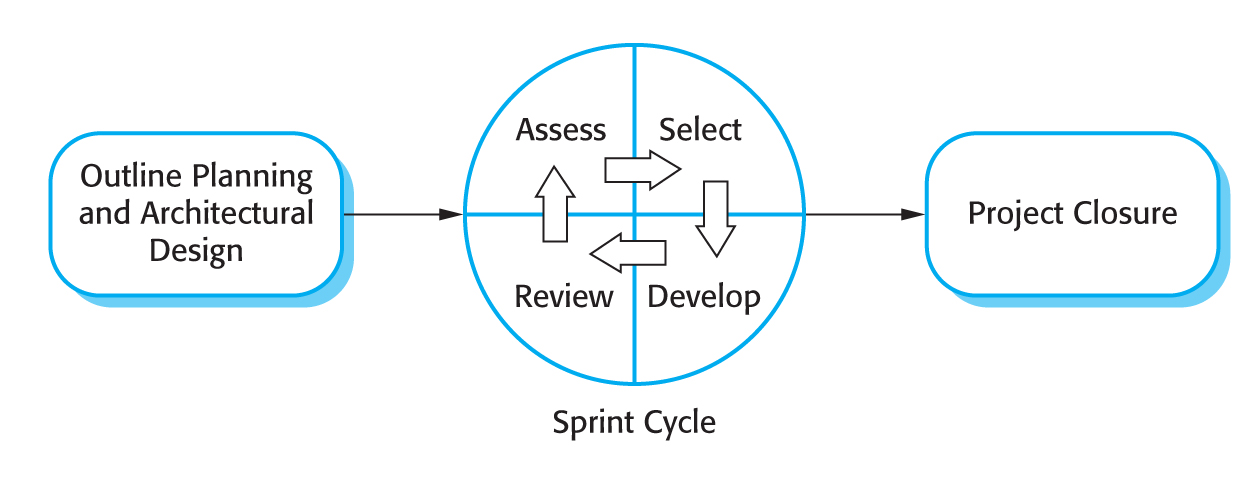
\includegraphics[width=120mm]{/content/SCRUM.jpg}\\
	  \caption{Scrum - the agile software development method}
\end{figure}

\textbf{1.Outline planning and architectural design}\\
This phase was concerned with general objectives and requirement analysis for the project and with designing software architecture. Former requirements specification section was very detailed and less suitable for agile development and therefore data flow sections have been omitted. Most of the underlying functional requirements have been left unchanged, but there have been some additions or improvements to them as the project development progressed. Some features have been renamed to convey better meaning and for consistency. There was a need for PEM's user interface changes with subsequent knowledge of an iPhone development acquired. \\ \\
\textbf{2.Sprint cycle}\\
Series of sprint cycles followed the previous phase where each cycle developed an increment of the system. Cycles had lengths 1-4 weeks. At the beginning of each cycle, meeting with a customer/supervisor took place where features of both applications were assessed and selected for the development. First half of the meeting was used for reviewing already completed cycle. Details of the meetings in appendices show what has been assessed, selected and developed.\\ \\
\textbf{3.Project closure}\\
Project closure phase wraps up the project, produces required documentation and draws conclusions.


% Project plan
\clearpage
\section{Project plan}
\subsection{Project Outline}
The goal of the project is to develop a system that can estimate user's caloric expenditure and advice him/her about their personal wellbeing or about wellbeing of the planet.
The system is split into two parts. First part is concerned with development of the Personal Energy Meter (PEM), which is an iPhone application and second part is dealing with development of a web application (PEMWEBAPP). Implementation of PEMWEBAPP has two purposes. First, is to receive data from PEM and present them in better graphical way using all real estate of computer monitor. Second, to demonstrate skills acquired during a course of study.


% Project schedule
\subsection{Project Schedule}
There are several important milestones in this project and each of those has several key tasks that must be performed. More information is given in the phase plan.
The main milestones for the project include:

\begin{itemize}
\item \textbf{General research} of the problem the project is concerned with, and production of the project plan overall (including the 
creation of this document as a guideline for the rest of the project, as well as being used 
as a general schedule). 



\item \textbf{Requirements Analysis}, aimed at finding all ambiguities, 
and determining exactly what the customer/user wants. This will include a decision on which 
design model to use.



\item \textbf{High Level Architectural Design}, which will help to determine how the applications will be structured given the limits and freedoms determined within the requirements Analysis phase.

\item \textbf{Implementation}, the stage in which the actual software systems are developed, using the designs created in previous stage. This phase will overlap with a design phase throughout whole development cycle to reflect on the agile approach.

\item \textbf{Evaluation of PEM} stage will be concerned with answering the questions whether the PEM solved given problem, how well it solved it and how accurately the solution matches with requirements. 
\end{itemize}


% Phase plan
\subsection{Phase plan}
\subsubsection{General research}
\begin{enumerate}
	\item Literature reviews
		\begin{enumerate}
			\item Research materials about GPS systems
			\item Research materials about Accelerometer
			\item Research materials about human wellbeing by physical activity
			\item Research materials about human calories expenditure
			\item Research materials about iPhone development and iOS SDK
			\item Research materials about Objective-C
			\item Research materials about Java EE 6, GlassFish  
			\item Follow the book “Projects in Computing and Information Systems”
		\end{enumerate}
	\item Meeting with customer/user
		\begin{enumerate}
			\item Meetings with project supervisor
			\item Getting feedback on application prototypes from friends
		\end{enumerate}
	\item Write the project proposal
\end{enumerate}


% Requirements Analysis
\subsubsection{Requirements Analysis - phase plan}
\begin{enumerate}
	\item Requirements discovery
		\begin{enumerate}
			\item User scenarios
			\item Customer/supervisor meetings
		\end{enumerate}
	\item Requirements classification and organization
		\begin{enumerate}
			\item Organizing and clarifying what has been gathered from customer/users
		\end{enumerate}
	\item Requirements prioritization and negotiation
		\begin{enumerate}
			\item Negotiating possible changes with customer/users and advice them on better suitable alternatives to meet the deadlines/budged
		\end{enumerate}
	\item Requirements specification
		\begin{enumerate}
			\item Clearing out ambiguities
			\item Producing a document which will act as a contract between customer and developer
		\end{enumerate}
	\item Write the interim report
\end{enumerate}


% Design
\subsubsection{Design - phase plan}
\begin{enumerate}
	\item PEM (Objective-C)
		\begin{enumerate}
			\item Architectural design for Profile manager
			\item Architectural design for Login with authentication
			\item Architectural design for Database (Apple's Core data)
			\item Architectural design for GPS tracking
			\item Architectural design for Live energy expenditure calculation
			\item Architectural design for Data transfer
		\end{enumerate}
	\item PEMWEBAPP (JavaEE)
		\begin{enumerate}
			\item Architectural for design for Login with authentication
			\item Architectural design for Profile view
			\item Architectural design for Database (MySQL)
			\item Architectural design for sessions view
			\item Architectural design for session details view
			\item Architectural design for Statistics

		\end{enumerate}

\end{enumerate}


% Implementation and Testing
\subsubsection{Implementation - phase plan}
The aim is to start as soon as possible without having to wait for total completion of solid software design – hence the agile development model. Modularization is used and attention is focused on some parts of the project, which will not change. In this way, implementation can start with only partial design. This strategy will be necessary in order to allow for any unforeseen complications in the design or implementation.
\begin{enumerate}
	\item Set up version control in Git
	\item PEM development
		\begin{enumerate}
			\item Implement Profile manager
			\item Implement Login with authentication
			\item Implement Database
			\item Implement GPS tracking
			\item Implement Live energy expenditure calculation
			\item Implement Data transfer
		\end{enumerate}
		Subtasks of the PEM development tasks will consist of:
		\begin{itemize}
			\item Interpreting architectural design diagrams in Objective-C language and trying to predict any deviations from the design.
			\item Coding the agreed design
			\item De-bugging
			\item Refactoring for better code structure
		\end{itemize}
	\item PEMWEBAPP development
		\begin{enumerate}
			\item Implement Login with authentication module
			\item Implement Profile view module
			\item Implement Database module
			\item Implement Statistics module
		\end{enumerate}
		Subtasks of the PEMWEBAPP development tasks will consist of:
		\begin{itemize}
			\item Interpreting architectural design diagrams in Java language and trying to predict any deviations from the design.
			\item Coding the agreed design
			\item De-bugging
			\item Refactoring for better code structure
		\end{itemize}
\end{enumarate}


% Evaluation
\subsubsection{Evaluation - phase plan}
\begin{enumerate}
	\item Evaluation of how well the systems meet customer/user requirement
		\begin{enumerate}
			\item There will be feedback received from the customer/user throughout the development process. Prototypes of the systems will be released in intervals to ensure meeting the requirements as closely as possible.
		\end{enumerate}
	\item Evaluation of how the systems are reliable
		\begin{enumerate}
			\item One of the extension features is to ensure the reliability of the PEM system by researching deep into iPhone Location Services and Accelerometer and utilizing full power of the hardware. Task of this part of evaluation will be proving the reliability of PEM in extreme conditions where two or more technologies might by interchanging in live energy expenditure monitoring mode.
		\end{enumerate}
	\item Evaluation of how the systems are accurate
		\begin{enumerate}
			\item In this part of the evaluation phase real biological results of obtained from health centers or fitness centers will be compared to those calculated by PEM. Results maybe obtained on request from staff or by measuring calorie expenditure of myself on treadmill. Note that it is also one of the extensions and not a priority to complete project.
		\end{enumerate}
\end{enumerate}


% Evaluation
\subsubsection{Testing - phase plan}
Carry out unit tests at the end of each sprint cycle when design of the systems is likely to change.


% Time estimates
\subsection{Time estimates}
Activity-on-node diagrams below show estimates of the time to complete both PEM and PEMWEBAPP systems. The figures have been estimated with constraints of learning new programming language in mind.

\begin{figure}[H]
  \centering
	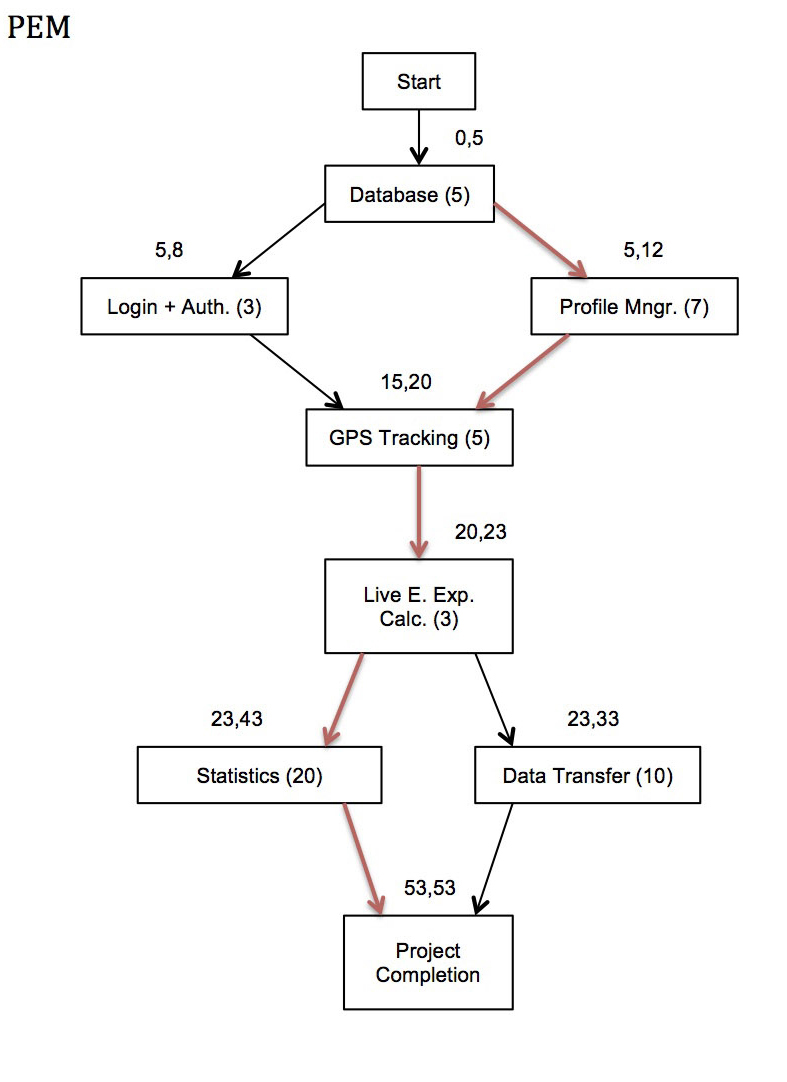
\includegraphics[width=120mm]{/content/PERTchart.jpg}
	  \caption{title}
\end{figure}

\begin{figure}[H]
  \centering
	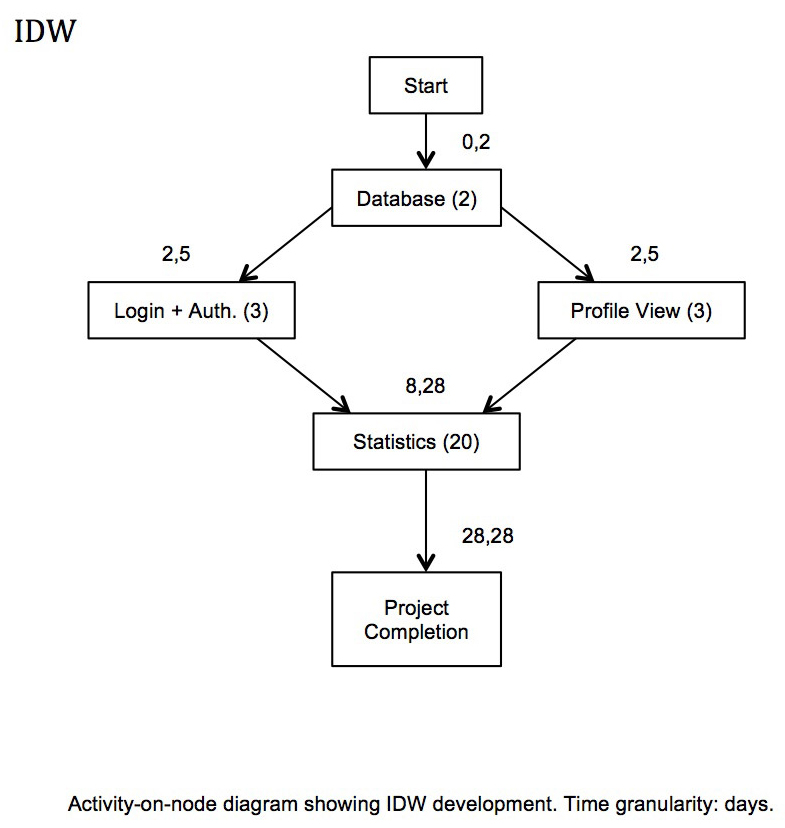
\includegraphics[width=120mm]{/content/PERTchart2.jpg}
	  \caption{title}
\end{figure}


% Requirements
\chapter{Requirements Analysis}

\section{Requirements discovery}
Requirements discovery has been carried out on three individuals. The project supervisor/main customer Martin and two friends of mine Tim and Richard. The requirements are very vague and high-level but refined throughout the stages of the Requirement Analysis.

\subsection{Collected scenarios}
\subsubsection*{Scenario 1}
Martin has a busy lifestyle in which time to rest and sleep is very precious. Therefore he would like to find a way of measuring and controlling the amount of energy he uses doing certain activities such as walking, running, cycling, working out in the gym or climbing stairs. As he is also very aware of the carbon footprint on the environment he would be interested in how much he could eliminate the emissions by changing his forms of transport.

\subsubsection*{Scenario 2}
Tim spends lots of hours in an office doing a sedentary job. To preserve his wellbeing he wants to know each day/week whether he had enough recommended physical activity. He would like to get accurate calorie expenditure results with healthy advices and recommendations directly on his iPhone or access it online via web page where he can log in, see all the results collected, graphically displayed using charts, and access and share other people's results to see general healthy trends.


\subsubsection*{Scenario 3}
Richard is a bodybuilder and therefore maintaining a strict workout program with enough rest each day is very important to him. As he is not a professional athlete he would appreciate some conventional way of keeping track of his calorie expenditure via heartbeat pulses while he works out in the gym. As a result, he would like to obtain very accurate data from which he could design or improve his workout program.

\section{Requirements classification and \\ organization}
On examination of all three scenarios and after consideration of the resources available for undertaking the project, following decisions have been made and presented to customer at one of the formal meetings: iPhone development will be used as this device was already available. (Developing for an iPhone also brings new challenges of learning new programming language, API and interesting development methods and models to this project.)

\subsubsection*{Product functionality}

The iPhone application should have following functionalities:

	\begin{itemize}
	\item Capture, categorize and process data (GPS, sound signal, accelerometer)
	\item Calculate calories expenditure using an Metabolic Calculation Model Model
	\item Calculate a carbon footprint
	\item Graphically output the results of the calculations
	\item Give recommendations on personal and planetary wellbeing
	\item Send data to remote website
	\end{itemize}

For accessing captured data from a computer an interactive dynamic website will be build. For the purposes of applying the knowledge of a Java language and Web Computing the website will be coded using Java EE 6 which is the industry standard for enterprise Java computing. This website should have following functionalities:
\begin{itemize}
\item Create and maintain user profiles
\item Receive and process data from the iPhone application
\item Graphically output results of calculations
\item Give recommendations on personal and planetary wellbeing
\item Share personal energy expenditure data with other users
\item Energy expenditure trends visualisation (personal, carbon footprint)
\end{itemize}
The classification and organization of the requirements discovery was a first important step of translating the high level user's scenarios to more technical and measurable units.

\section{Requirements prioritization and \\ negotiation}
Although the classification and organization phase of the requirements discovery laid down some understandable structure to the project, which is closer to implementation than vague user scenarios, the time constraint of the project became very apparent. Negotiations with the customer therefore had to take place in order to preserve prototype and final product release dates schedule.

\subsubsection*{Objectives after negotiation}
Primary:
	\begin{itemize}
		Design and develop the Personal Energy Meter (PEM), an iPhone application that 		should 	have following functionalities:
	\end{itemize}
	\begin{itemize}
		\begin{itemize}
			\item Capture and process GPS data of five activity domains (Walk, Run, Car, Bus and Train)
			\item Calculate calories expenditure using an Metabolic Calculation Model Consumption Model
			\item Calculate a carbon footprint
			\item Graphically output results of the calculations
			\item Give recommendations on personal and planetary wellbeing
			\item Send data to remote website
Design and develop an interactive website which should have following functionalities:
			\item Create and maintain user profiles
			\item Receive and process data from the PEM, an iPhone application
			\item Graphically output results of calculations
			\item Give recommendations on personal and planetary wellbeing
		\end{itemize}
	\end{itemize}
Extensions: 
	\begin{itemize}
		\begin{itemize}
			\item More precise GPS data processing by PEM
			\item Live GPS data categorization (walking, driving car, running, using public transport)
			\item iPhone in-built headphones microphone integration for capturing the heartbeat (for estimating energy expenditure indoors where high volume of energy can be used for example in the gym or climbing stairs)
			\item Validation of the Energy Consumption Model with real biomedical measurements
			\item Improve accuracy and reliability of capturing the GPS data
			\item Share the personal energy expenditure data with other users
			\item Energy expenditure trends visualization (personal, carbon footprint)
		\end{itemize}
	\end{itemize}
Splitting the project requirements, by negotiating with the customer, into two categories (Primary, Extensions) reduced a development overhead, which wasn't apparent in the initial stages of formal meetings. The negotiation gave both stakeholders more clear understanding of what can be achieved within designated time of the project (or how much the customer can have for what s/he paid). The development company has however offered the customer, for keeping a good customer relations, an implementation of some or all ‘Extensions' if time allows.


% Requirements Specifications
\section{Requirements Specification}
Requirements have been captured in a Requirements Document (RD), which forms an official statement of what the system developer (myself) should implement.\\ \\
PEM is a small iPhone application that solves the problem of knowing person's energy expenditure in everyday life. It monitors person's movements and from data obtained it estimates the amount of calories a person burned in various activities. As an output, PEM provides a graphically aided representation of results together with healthy recommendations. PEMWEBAPP is a website which solves a problem of having to interact with limited real estate of an iPhone screen and present the results in better graphical way on computer monitor.

\subsection{User requirements definition}
The PEM shall create user profile and shall provide profile view where updating user's profile data is possible. The PEM shall provide GPS tracking for five activity domains (Walk, Run, Car, Bus and Train) and shall be calculating calorie expenditure and carbon footprint, and shall have an option to save the activity tracking as a session into persistent store for later retrieval. The PEM shall have a session details view where retrieved information will be displayed and emphasized by graphical aids. The PEM shall have an upload feature for uploading the data (profile and sessions) into online PEMWEBAPP. The PEM shall provide recommendations on personal and planetary wellbeing and have user authentication feature.\\ \\
The PEMWEBAPP shall manage user profiles, display profile and profile's sessions and shall provide sessions details view. The PEMWEBAPP shall provide a delete profile button for deletion of the profile and all its sessions. The PEMWEBAPP shall also have a statistics view where each session will be depicted on a line chart showing calorie expenditure and carbon footprint data. The PEMWEBAPP shall provide recommendations on personal and planetary wellbeing and have user authentication feature.


\begin{figure}[H]
  \centering
	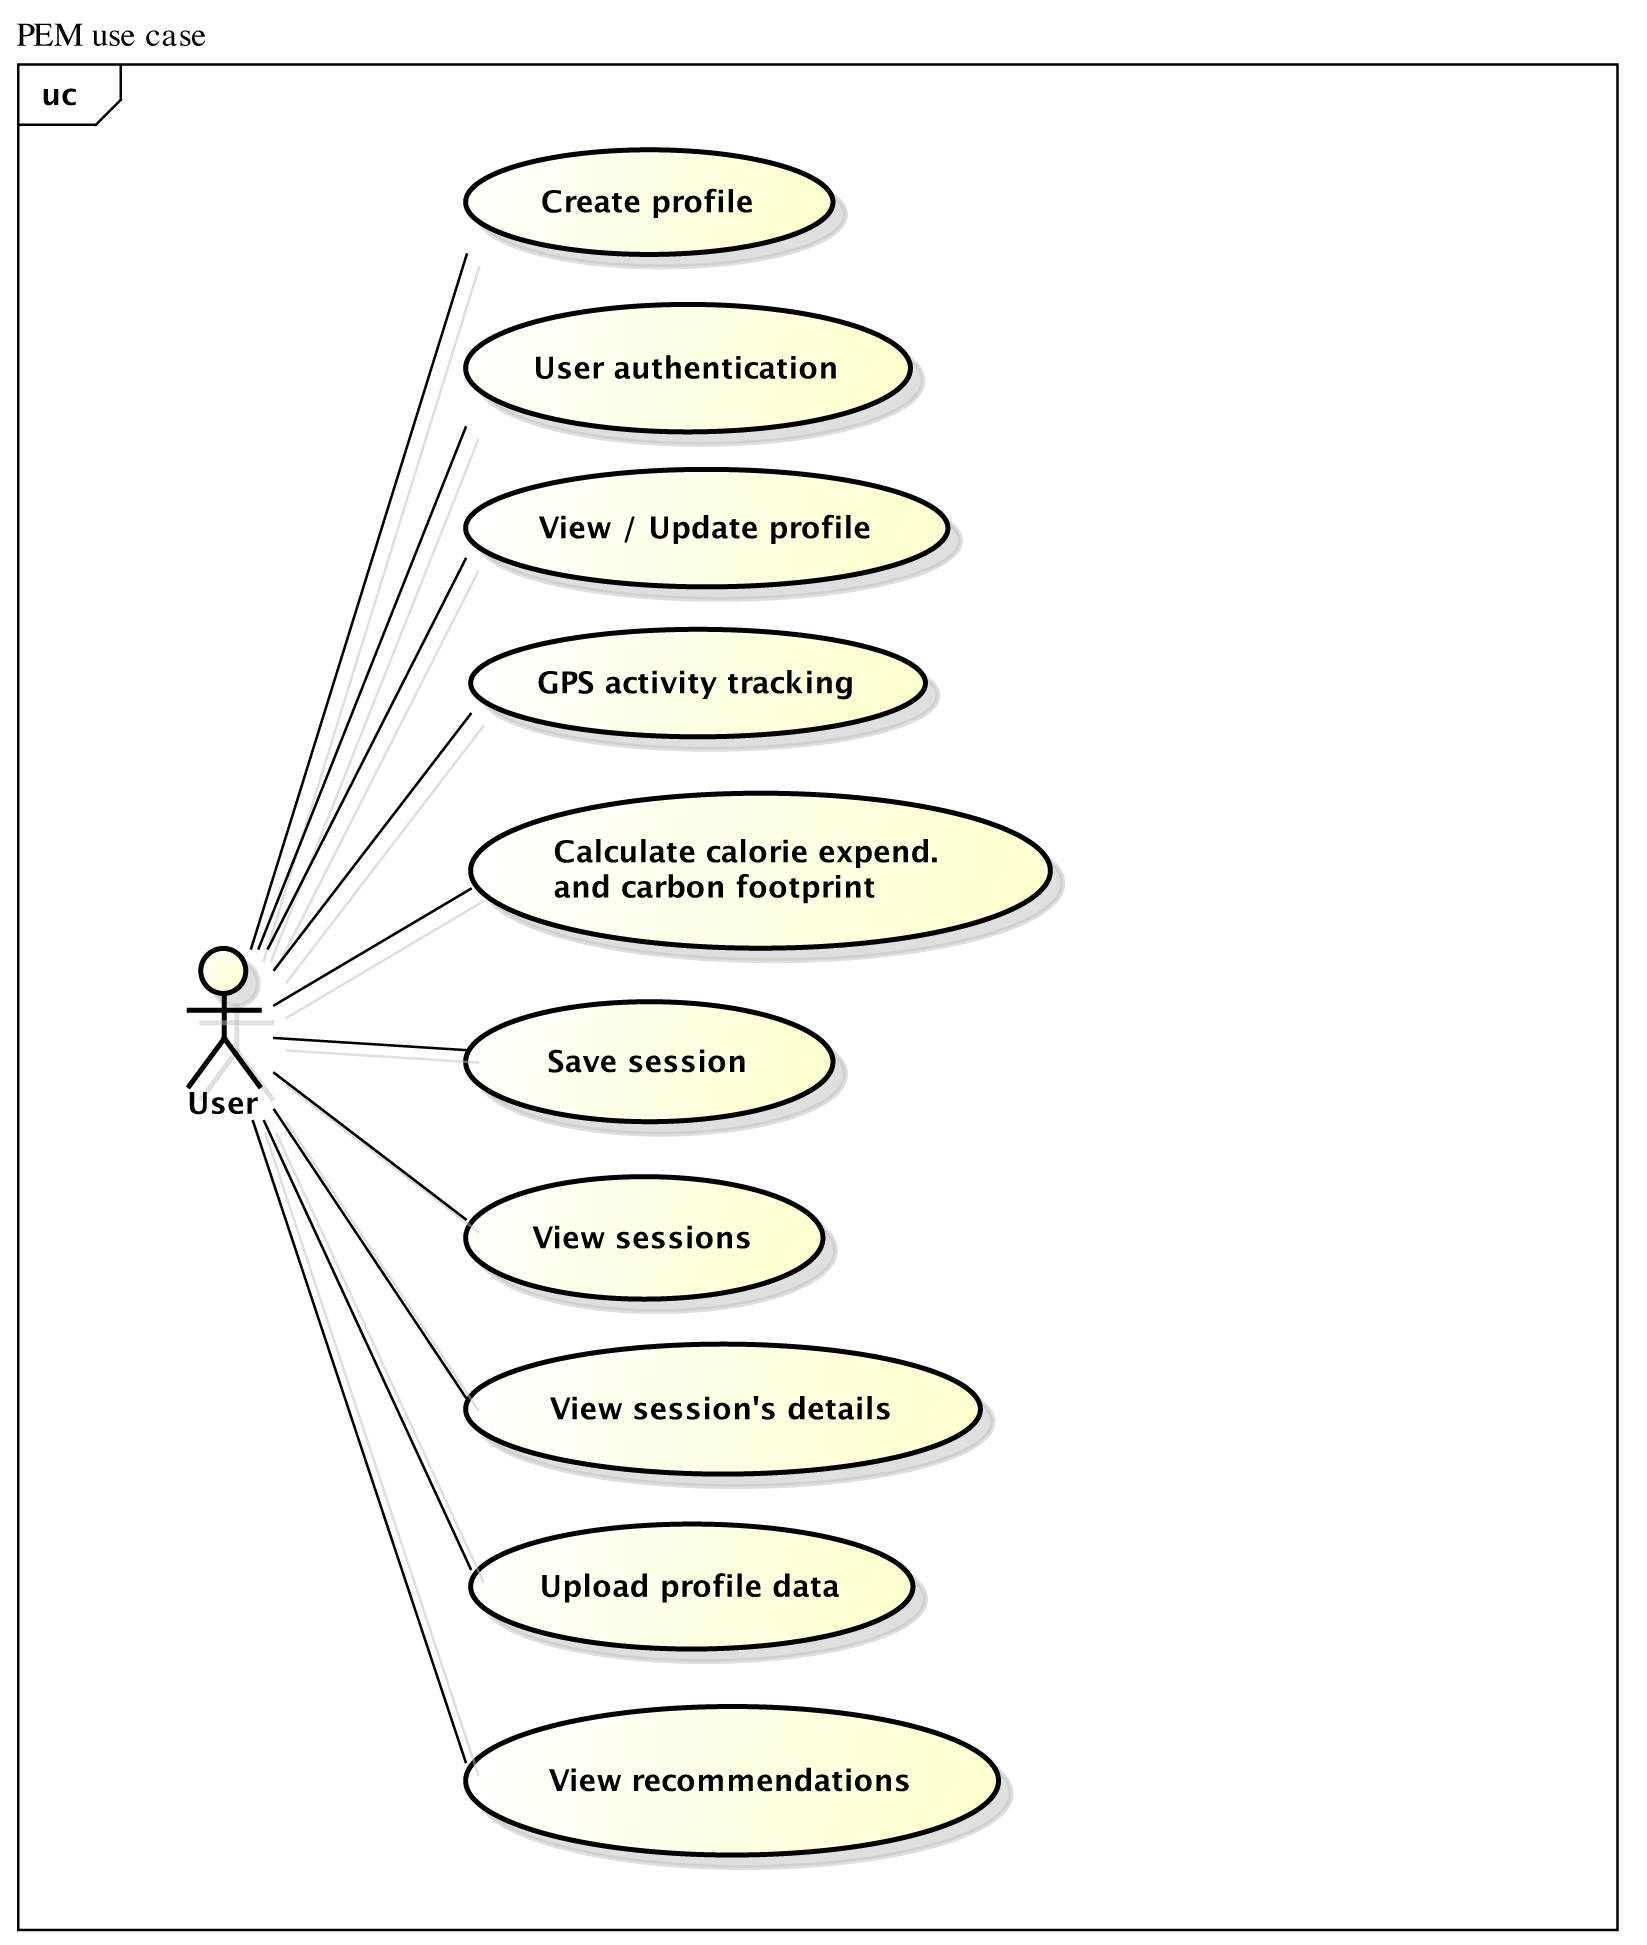
\includegraphics[width=120mm]{/content/PEM_use_case.jpg}
	  \caption{title}
\end{figure}

\begin{figure}[H]
  \centering
	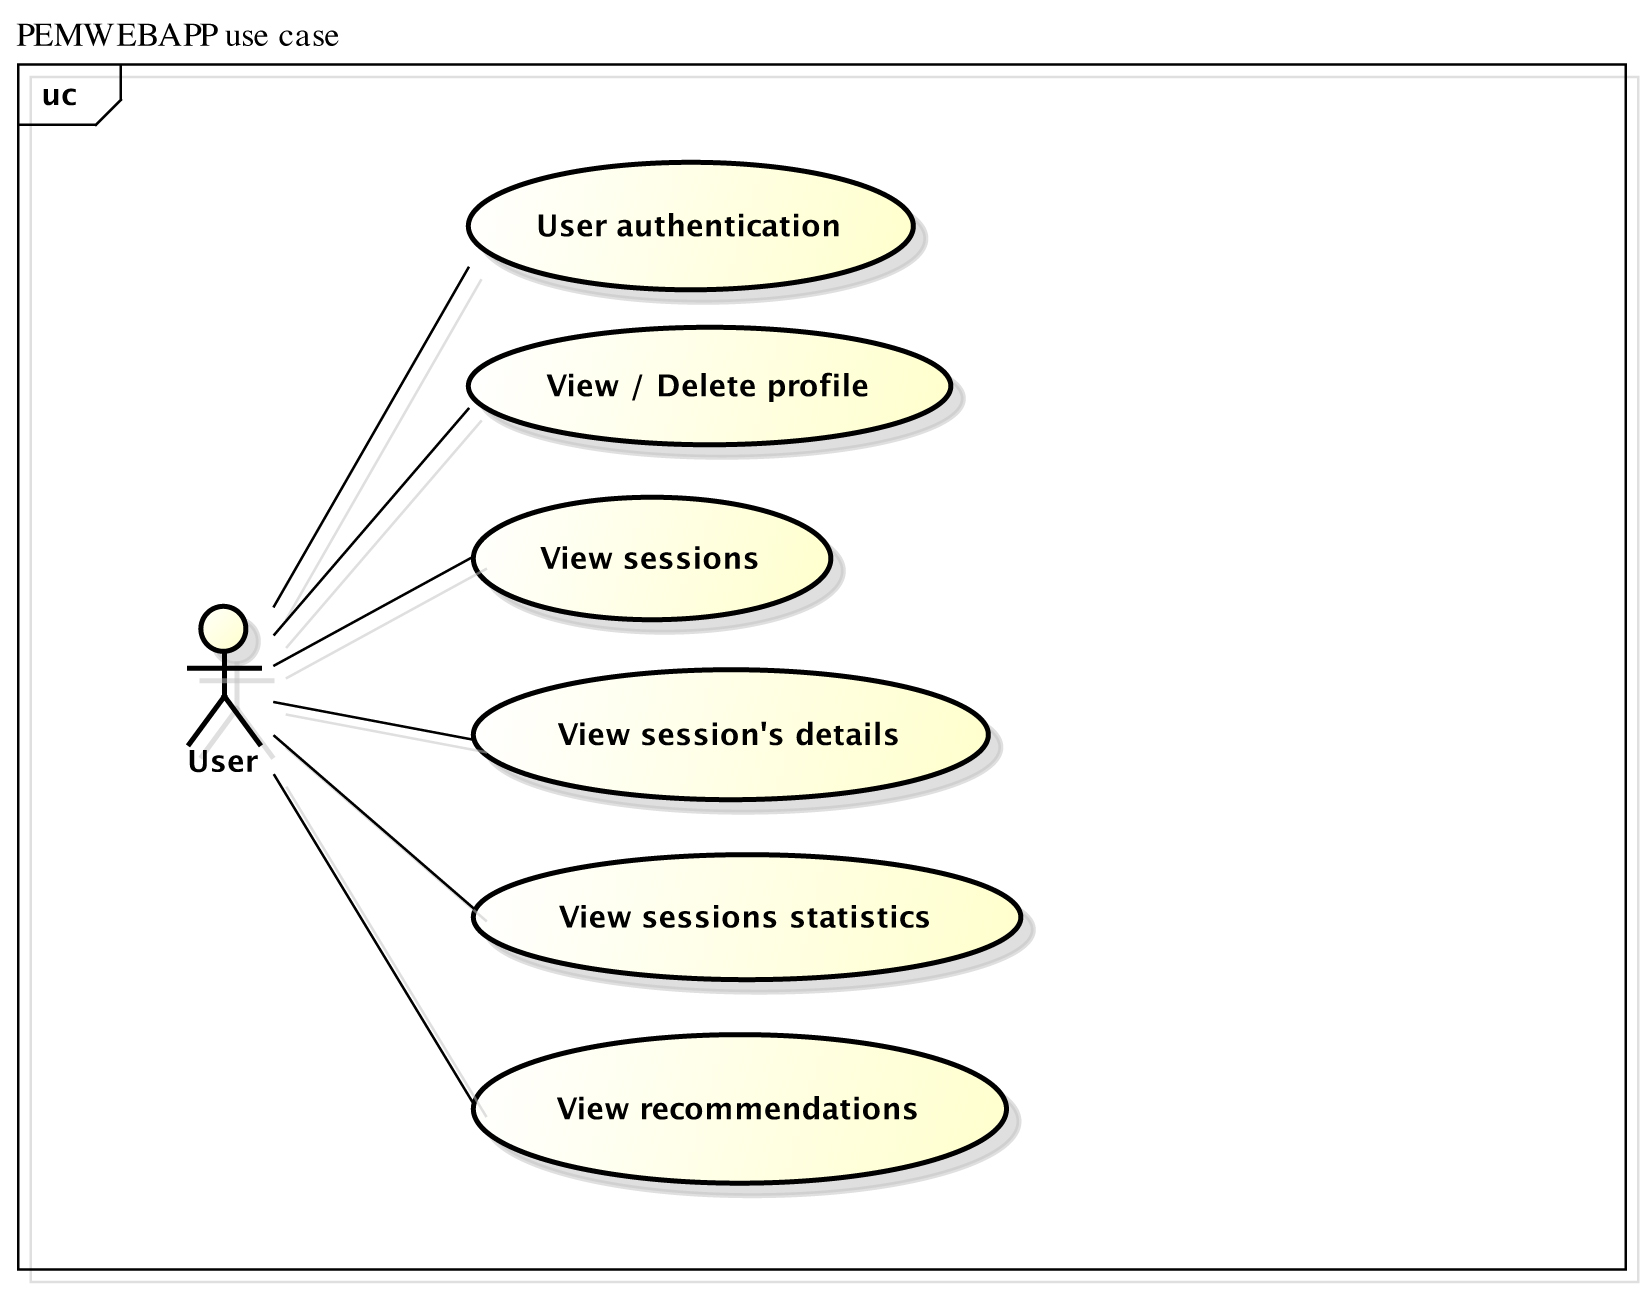
\includegraphics[width=120mm]{/content/PEMWEBAPP_use_case.jpg}
	  \caption{title}
\end{figure}


% Functional requirements
\subsection{System requirements specification}
\subsubsection{Functional requirements}
Personal Energy Meter (PEM)\\ \\
\textbf{1. Create Profile}\\
This feature shall provide the ability to create a new profile on the PEM. It is the first thing a user must do to begin using PEM. Its main function is to set up a new profile with personal details such as email and password. Email shall act as a username and must be unique. Password must be at least 4 characters long, no longer than 20 and must contain at least one numeric character. No special characters are allowed.\\ \\
\textbf{2. Log-in}\\
This feature shall allow the user to log in to the existing profile on PEM. When choosing to log in, the user is asked to enter his/her email and password. After a successful authentication the activity screen appears.\\ \\
\textbf{3. Edit profile}\\
This feature shall allow the user to edit his/her personal details on PEM. When the user is logged in he/she should be able to edit his/her personal details such as adding first and second name or change a body weight. There shall be a constraint on editing the email to preserve correct transfer of data to the appropriate profile on the remote server (email is unique and represents a profile). Password must be at least 4 characters long, no longer than 20 and must contain at least one numeric character. No special characters are allowed.\\ \\
\textbf{4. Delete profile}\\
This feature shall allow user to delete his/her profile from the PEM. Users not wanting to keep their profile for various reasons or wanting to start from scratch should have an option to delete their profile with all the data gathered. This operation should only affect the PEM system. Users should be able to still access their profile online to see all of the data and results. Deleting online profile shall be done in the PEMWEBAPP.\\ \\
\textbf{5. Start tracking}\\
This feature shall allow user to start his/her energy expenditure or carbon footprint monitoring. By pressing the Start button, the iPhone device shall start to receive GPS data and at the same time shall perform live calculations of calories burned and/or CO2 emissions calculations. The Location Services on iPhone have to be enabled in order for PEM to receive any GPS data.\\ \\
\textbf{6. Stop tracking}\\
This feature shall allow user to stop his/her energy expenditure or carbon footprint monitoring as well as to stop receiving GPS data. By pressing the Stop button, user should be prompted if he/she whishes to save a session. Monitoring needs to be in progress in order for Stop to have an effect and ask about saving the data.\\ \\
\textbf{7. Pause tracking}\\
This feature shall allow user to pause their energy expenditure or carbon footprint monitoring as well as to stop receiving GPS data and resume it all again.\\ \\
\textbf{8. Google maps and tracking information}\\
This feature shall allow user to see live position on Google maps and GPS data as they are received in intervals (every second). Data such as horizontal accuracy, elevation, distance traveled, grade, speed, time, VO2, Calories and CO2 emissions should be displayed under map view. The map view should be zoom-able and follow user current position.\\ \\
\textbf{9. Sessions view}\\
This feature shall allow user to navigate through all saved sessions (related to his/her profile) and choose desired session to show in the details view. This view shall pull limited session data from the PEM's database to show only a session name and timestamp. User should be able to delete the session from this view by swiping the session cell or by using an edit button.\\ \\
\textbf{10. Session details view}\\
This feature shall allow user to see session details. View shall contain all information gathered by GPS tracking and also results of calculations (session name, timestamp, activity, horizontal accuracy, elevation, distance traveled, grade, speed, time, VO2, Calories and CO2 emissions). Most important data such as total calorie expenditure or total CO2 emissions should be emphasized using graphical aids.\\ \\
\textbf{11. Recommendations}\\
This feature shall provide the most important information and facts about a type of activity monitored. For example if the Walk or Run activity has been monitored and stored the feature should provide relevant information about recommended amount of daily calorie intake and guidelines on how to lose or maintain weight. For sessions, which monitored activity such as Car, Bus or Train, recommendations should advice user about ways on how to reduce carbon footprint.\\ \\
\textbf{12. Upload profile}\\
This feature shall upload user's profile with all sessions to the remote PEMWEBAPP. This operation should be available at any time after user profile has been created.\\ \\
\textbf{13. Log-out}\\
This feature shall log user out from the PEM.\\ \\
\subsubsection{Functional requirements}
PEM Web Application (PEMWEBAPP)\\ \\
\textbf{1. Log-in}\\
This feature shall allow the user to log in to the existing profile on PEMWEBAPP. When choosing to log in, the user is asked to enter his/her username and password. After a successful authentication a profile view appears.\\ \\
\textbf{2. Profile page}\\
This feature shall allow user to see his/her profile. Information such as first and last name, email and body weight should appear as user entered them in the PEM. Password shall not show in this view. None of the information shall be editable.\\ \\
\textbf{3. Delete profile}\\
This feature shall allow a user to delete his/her profile from the PEMWEBAPP. Users can delete unwanted profile together with all the data gathered. This operation can't be undone.\\ \\
\textbf{4. Sessions page}\\
This feature shall allow user to navigate through all uploaded sessions (related to his/her profile) and choose desired session to show in the details view. View shall pull limited session data from the PEMWEBAPP's database to show only a session name and timestamp. None of the information shall be editable.\\ \\
\textbf{5. Session details page}\\
This feature shall allow user to see session details. View shall contain all information as they were stored by PEM (session name, timestamp, activity, horizontal accuracy, elevation, distance traveled, grade, speed, time, VO2, Calories and CO2 emissions).\\ \\
\textbf{6. Statistics page}\\
This feature shall allow user to see statistics of recorded activities in a line chart. Line chart shall show Calories burned and CO2 emissions for each session.\\ \\
\textbf{7. Recommendations}\\
This feature shall provide the most important information and facts about a type of activity monitored (very similar to PEM's recommendation feature with exception that it should be accessible from the statistics page rather than session details page).\\ \\
\textbf{8. Log-out}\\
This feature shall log user out from the PEMWEBAPP.\\ \\


% Non-functional requirements
\subsubsection{Non-functional requirements}

\begin{enumerate}
	\item Product requirements\\ \\
	Following are the Human-Computer-Interaction guidelines against which the PEM application should be evaluated. PEMWEBAPP should be also evaluated against these guidelines where appropriate.\\
	\begin{enumerate}
		\item Usability goals
		\begin {enumerate}
			\item Effectiveness: energy and calorie estimates must be of the highest accuracy possible for the application to be effective.
			\item Efficiency: the application needs to have immediate response and perform live calculations 
			\item Safety: safe storage and data transfer is critical for this type of application and users should not have to worry whether their data is safe.
			\item Utility: PEM should be build correctly and do only what is its intention to maximize utility. There should be no adverts or misleading content.
			\item Learnability: PEM must be easy to learn. Following Apple's Human Interface guidelines, the Norman's design principles and using well identifiable buttons and other UI controls will be necessary to achieve this. Furthermore, the application must be simple to use for users who are complete novices. It must have step-by-step instructions for initial setup, tracking and profile upload. Option selection should be constrained to prevent wrong choices. There is no need for extra flexibility or shortcuts for advance users because the PEM will be very easy to use with a limited number of features.
			\item 6. Remembering: PEM will be a multiscreen application. To maximize recognition rather than recall, each screen will have unique elements wrapped into consistent design used throughout the application.\\
		\end{enumerate}

		\item Experience goals
		\begin{enumerate}
			\item Satisfaction: the PEM should invoke satisfying feeling when it proofs itself effective.
			\item Enjoyment, Fun and Entertainment: PEM should strive for this goal by using simple, responsive and swift GUI. The session details view could be a good place investing into creativity.
			\item Helpfulness: PEM should deserve this goal by being reliable and delivering correct data when needed. Users then can make wise decisions based on application's recommendations.
			\item Motivation: PEM should be able to motivate people to reduce carbon footprint and motivate them to live healthily.
			\item Aesthetic: PEM should have aesthetic qualities if the design will follow the design principles and human interface guidelines.
			\item Support: PEM should have a help section which is easy accessible and readable.
			\item Reward and Emotional fulfillment: Users of PEM should be able to feel rewarded and emotional fulfilled for helping to improve their health and planetary wellbeing.\\
		\end{enumerate}
		
		\item User Interfaces:
		\begin{enumerate}
			\item PEM user interface shall be made of various forms, views and pickers all of which are standard iPhone UI components. It should consist of following screens (Login, Activity, Profile, Tracking, Save session, Sessions and Session details). Tab bar at the bottom of the GUI will allow switching between individual screens.\\
			\item PEMWEBAPP user interface shall be made of Java Servlet Faces and third party PrimeFaces components, which support AJAX for better user experience. It should consist of the following pages (Login, Profile, Sessions, Session details and Statistics). To navigate through the website, standard top-horizontal navigation consisting of links shall be used.\\
			\end{enumerate}
	
		\item Efficiency requirements
		\begin{enumerate}
			\item PEM's monitoring feature should be able to pin point most accurate current position within 10-20 sec outdoors.\\
			\item iPhone's inaccurate altitude data received from GPS shall be replaced with accurate elevation data. For this purpose the Google Elevation API shall be used.\\
		\end{enumerate}

		\item Security requirements
		\begin{enumerate}
			\item Both applications shall use hashing of stored data.
			\item Use secure data transfer.
			\item Use user authentication.\\
		\end{enumerate}
	\end{enumerate}

	\item Organizational requirements

		\begin{enumerate}
			\item Platforms and languages
			\begin{enumerate}
				\item PEM – Apple (Objective-C)
				\item PEMWEBAPP – Oracle (Java Enterprise Edition)
				\item PEM - SQLite database wrapped by Core Data
				\item PEMWEBAPP - MySQL database\\
			\end{enumerate}
			
			\item Interoperability
			\begin{enumerate}
				\item PEMWEBAPP shall be implemented as a REST service so that iPhone can communicate with it using GET and POST commands.\\
			\end{enumerate}

			\item Metabolic and carbon footprint calculations
			\begin{enumerate}
				\item PEM shall make use of the ACSM's Metabolic Calculation Handbook for calculating VO2 and consequently calculating of Calorie expenditure.
				\item PEM shall make use of the Carbon Trust's passenger transport conversion factors for calculating carbon footprint.\\
			\end{enumerate}
		\end{enumerate}
		
		\item External requirements
		\begin{enumerate}
			\item The PEM must be built correctly to pass Apple's requirements for application distribution in the App Store. Both PEM and PEMWEBAPP must comply with the Code of Conduct and the Code of Good practice and must use secure file transfer to online website, cannot violate personal privacy by broadcasting user's location and location history must be stored securely.
		\end{enumerate}
	\end{enumerate}
	

% System models
\subsection{System models}
Following models are activity diagrams of both applications. First diagram was created in the initial stages of development where as the second diagram was created in later stages of development where more knowledge and experience has been acquired.


\begin{figure}[H]
  \centering
	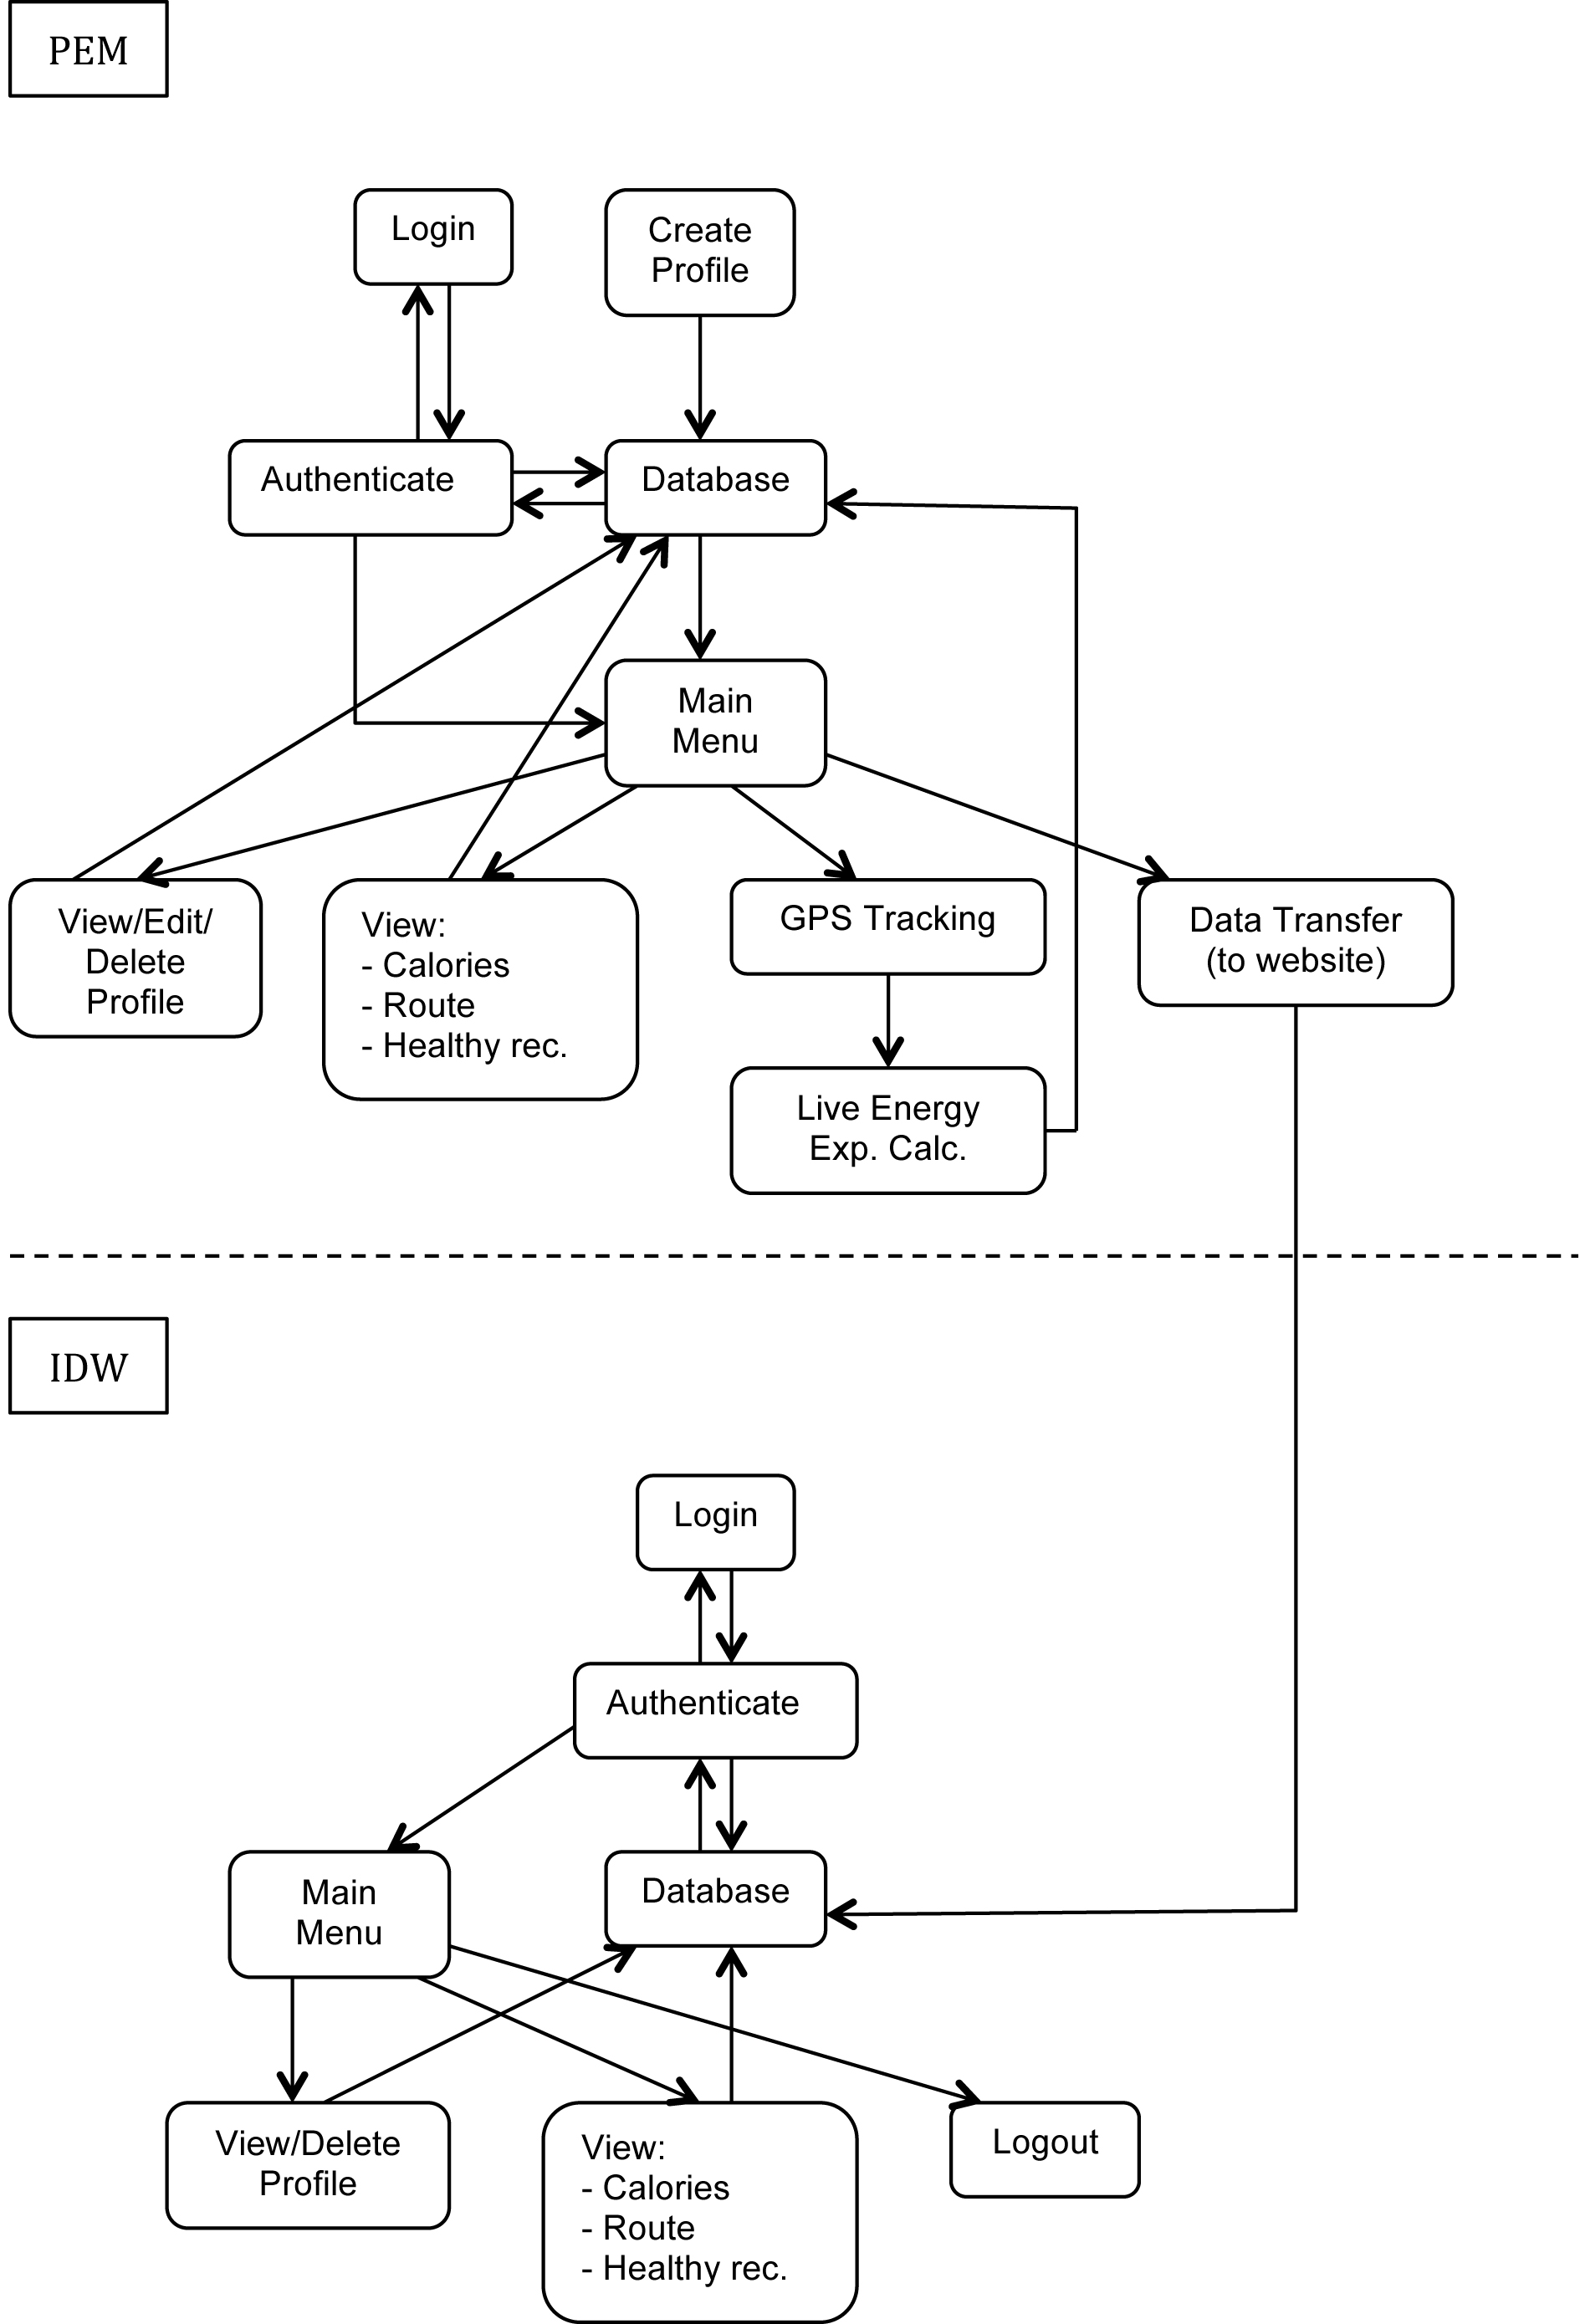
\includegraphics[width=120mm]{/content/InitialObjectDiagram.jpg}
	  \caption{Initial object diagram showing interactions between PEM and IDW (aka. PEMWEBAPP)}
\end{figure}


 \begin{figure}[H]
 \begin{sideways}
 \begin{minipage}{19cm}
	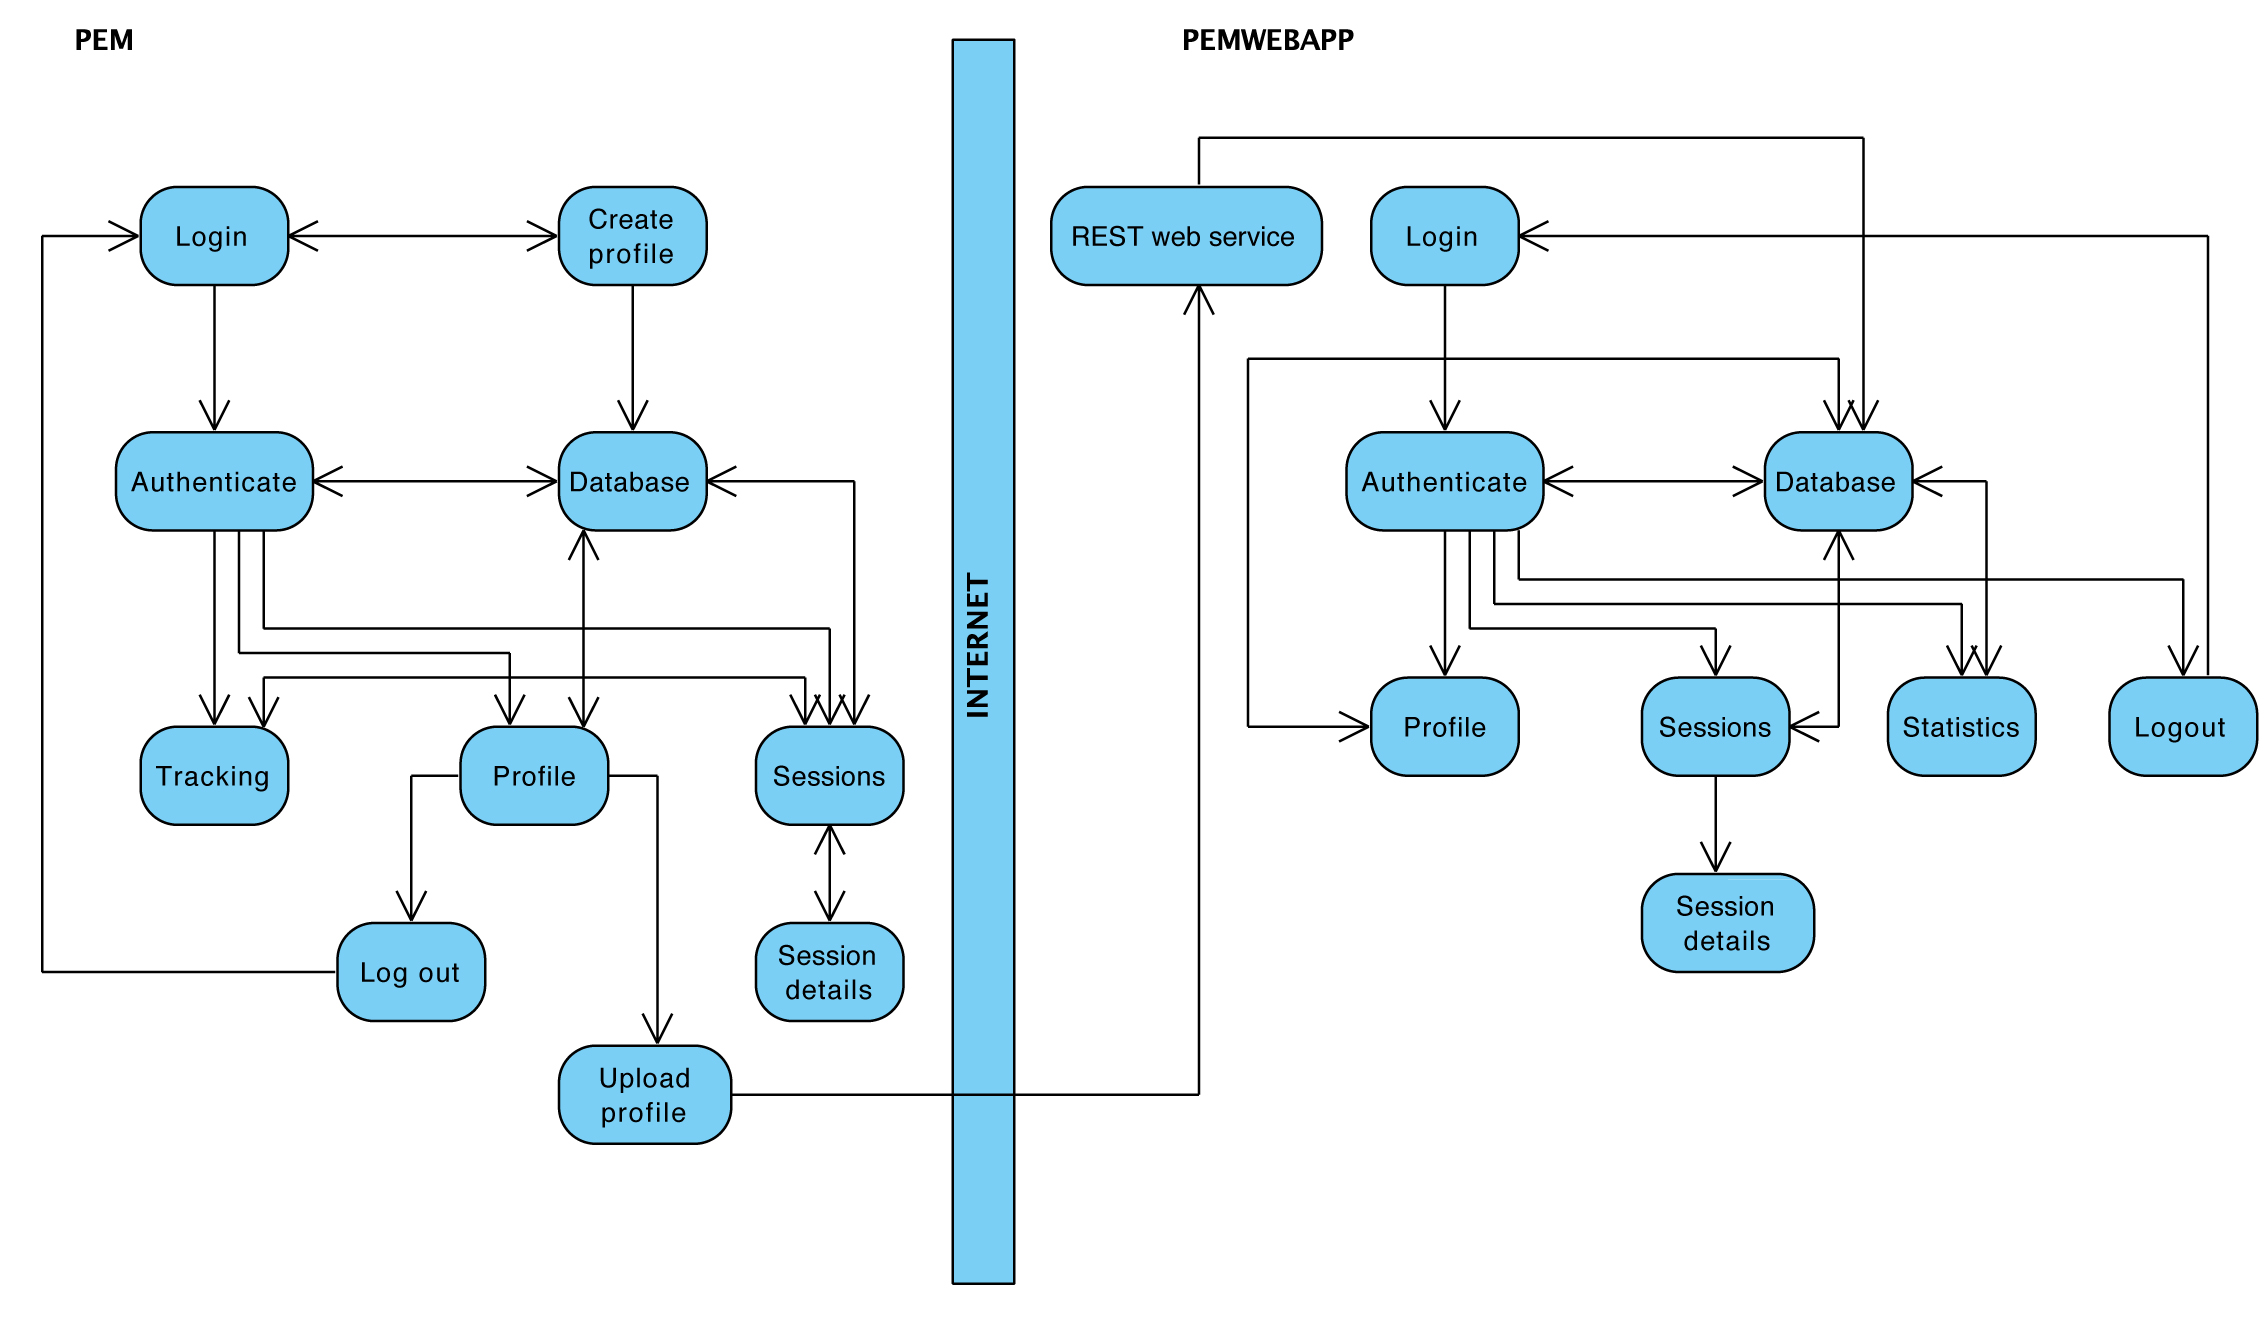
\includegraphics[width=200mm]{/content/SystemsObjectDiagram.jpg}
	  \caption{Improved object diagram showing interactions between PEM and PEMWEBAPP in mid stages of development}
 \end{minipage}
 \end{sideways}
 \centering
 \end{figure}


% Design and Implementation
\chapter{Design and Implementation}
\section{Introduction}
As already mentioned, the agile software development was most appropriate for this project and therefore there was no solid design in the initial stages of PEM and PEMWEBAPP development.
The design was being developed continuously by getting ideas, proposing solutions, and refining these solutions as information became available during the sprint cycles. Many times there was a need to backtrack and re-design when problems arose [REF – Chapter 7.1]. Paper sketches and Xcode's storyboards were the only key documents from which the development initiated. There was a time when vast majority of the PEM had to be redesigned as knowledge of an iPhone development improved and having a detailed design beforehand would be a waste of time.\\ \\
Initial paper sketch scan….\\
Initial storyboard image….\\ \\
Some inspiration of how the PEMWEBAPP might look like or what data might be useful to collect came from fitbit.com and bodymedia.com. Both companies are well established in areas of estimating personal energy expenditure.

\begin{figure}[H]
  \centering
	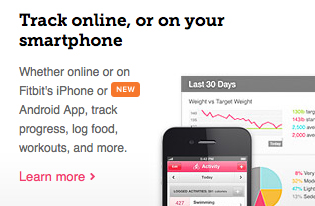
\includegraphics[width=120mm]{/content/fitbit.jpg}
	  \caption{One of the features promoted by Fitbit.com}
\end{figure}

\begin{figure}[H]
  \centering
	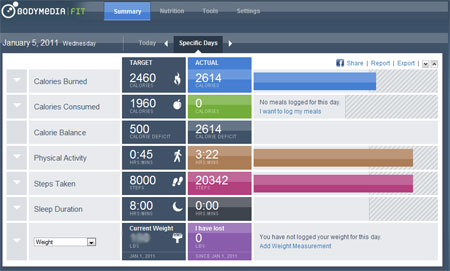
\includegraphics[width=120mm]{/content/bodymedia.jpg}
	  \caption{Dynamic website of Bodymedia.com}
\end{figure}

\clearpage
\section{Building a simple iPhone application}
Project has initiated by first meeting, which focused on chosen project topic. Discussion covered available hardware and software and was aimed on encouragement to learn a new programming language. First stage of the Scrum method, the planning, included gathering requirements, getting to know an iOS development and Xcode IDE, registering in an Apple Developer Program and configuring a computer to be able to deploy applications to an iPhone. First sprint cycle was launched as soon as basic knowledge of an iPhone development has been acquired and some requirements gathered, resulting in creation of a simple iPhone application.

\begin{figure}[H]
  \centering
	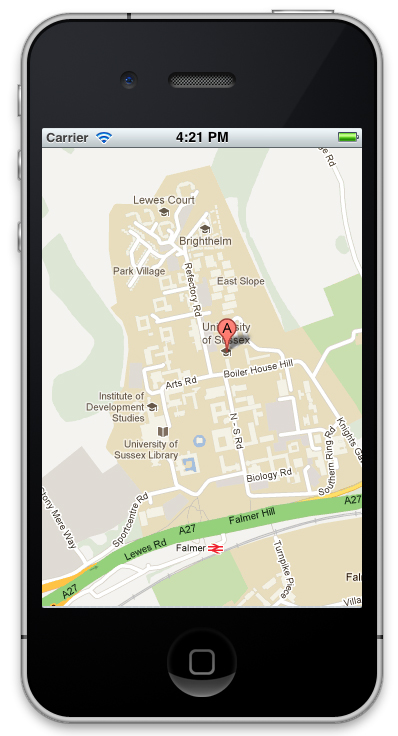
\includegraphics[width=50mm]{/content/simpleiPhoneApp.jpg}
	  \caption{Simple iPhone application}
\end{figure}


The application was able to pinpoint user's current position and show it in a map view. To build this simple application a fundamental iPhone development design pattern had to be used, the MVC pattern. A view was built in the Xcode's Interface Builder and wired up to the application's logic. This logic was written in an ordinary class, which was a subclass of a UIViewController (User Interface View Controller) providing more functionality. At this stage there was no persistence store to persist application's data thus the Model part of the MVC pattern wasn't fully utilised. Figures below show iPhone's application key objects and how the functionality was wired up to the user interface.


\begin{figure}[H]
  \centering
	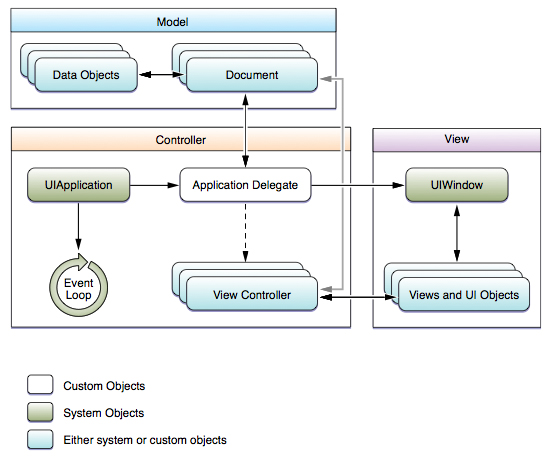
\includegraphics[width=120mm]{/content/iOSAppKeyObjects.jpg}
	  \caption{REF Apple programming guide}
\end{figure}

\begin{figure}[H]
  \centering
	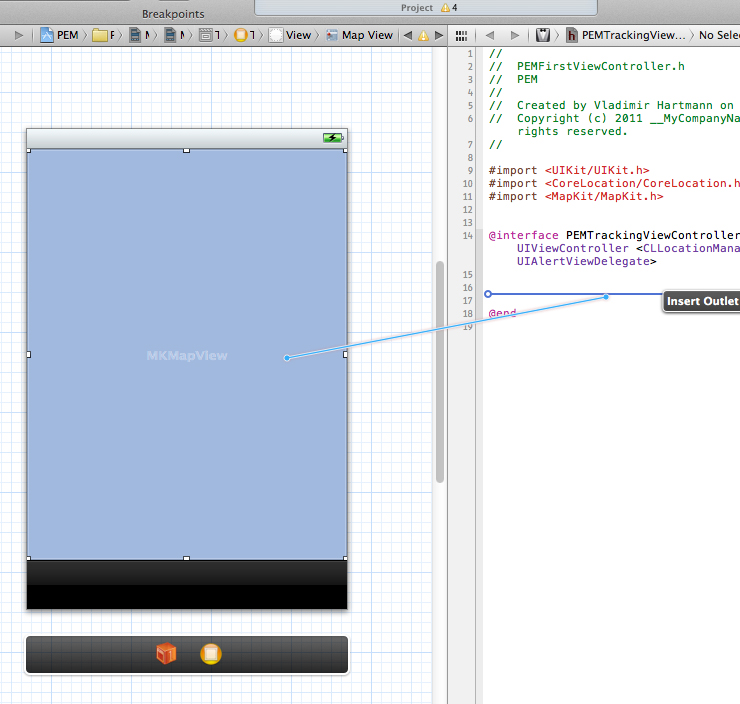
\includegraphics[width=100mm]{/content/iPhoneApp-wiringAction.jpg}
	  \caption{Wiring up functionality to user interface}
\end{figure}


\clearpage
\section{Improving the simple iPhone application}
Demonstration of the simple iPhone application to the customer/supervisor completed the first sprint cycle and at the same time initiated a next one with emphasis on importance to write as much code as possible without worrying about detailed design. Main tasks of this cycle were further programming of the simple iPhone application, a research of previous attempts to build PEM, study of the Apple's Human-Interface guidelines and gathering a literature about utilising location services on iPhone and about GPS in general. As a result a GPS application was built that could capture location coordinates of current position and display them on iPhone screen.


\begin{figure}[H]
  \centering
	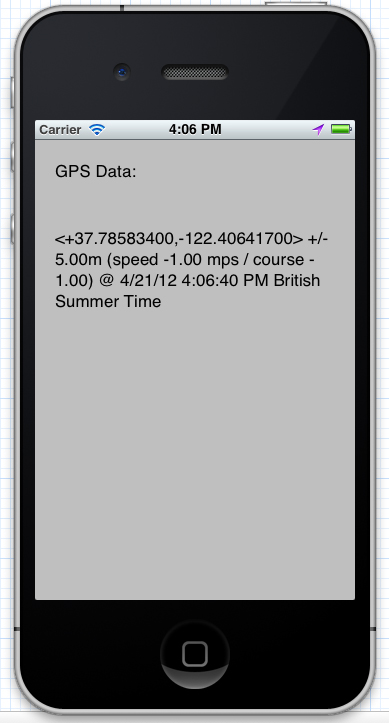
\includegraphics[width=50mm]{/content/FirstGPSApp.jpg}
	  \caption{The simple iPhone application extended by GPS functionality}
\end{figure}


\clearpage
\section{Utilizing Apple's Core Data and Core Location}
Following two sprint cycles were mostly concerned with learning iPhone data persistence and location services.

There are many ways how to persist data on iPhone devices such as using property lists, archiving, directly interfacing with SQLite or using the Core Data framework. First two approaches were not very suitable for storing big amounts of data. Utilising the SQLite and directly interfacing it would work just fine, but Apple introduced more elegant solution of working with relational databases. Core Data allows programmer to think of their data model in terms of objects/entities and their relationships. This is important as the code can retrieve and manipulate this data on a purely object level with simplified fetch requests and there is no need to work with relation schemas and complicated query language which can introduce errors or security issues.
Because receiving location data is not enough to estimate user's calorie expenditure it was necessary to learn about Core Location.
Core Location is an iOS framework, which allows easy access to the iPhone's GPS. Precise Apple's description is:
“The Core Location framework lets you determine the current location or heading associated with a device. The framework uses the available hardware to determine the user's position and heading. You use the classes and protocols in this framework to configure and schedule the delivery of location and heading events. You can also use it to define geographic regions and monitor when the user crosses the boundaries of those regions.”\\ \\
% [REF]
It is important to mention that during assessments and reviews of these sprint cycles discussion on how to improve accuracy was also relevant. GPS hardware in Apple's devices as well as in any other mobile device currently on market is well known for producing inaccurate altitude data. This is mostly due to position of satellites, which calculate the altitude \[REF http://weather.gladstonefamily.net/gps_elevation.html\]. One of the suggested project extensions was implementation of signal processing for heart bean measurements. This technique, if implemented correctly, would prove very accurate for estimating calories expenditure as it could be used in situations where user's position is not changing much but calories expenditure is being high e.g. working out in a gym. The signal processing approach is though big subject on its own and soon became apparent that realisation of this technique would need far more time than allocated for final year project.\\ \\
At the end of the cycles a first PEM prototype was built which featured everything previously built so far plus measuring the distance. Extensive GPS data filtering had to be done in order to work with gathered data. For example lots of invalid location data was received during Core Location initialization with values differing up to 500m. These had to be filtered out by checking their timestamps or specifying a threshold. Core Location uses caching for storing previously gathered data to prevent frequent use of the GPS. For real time application such as PEM however, this would cause old data to be processed in later implemented calculations. Compromise had to be made to trade battery life for up-to-date data.


\begin{figure}[H]
  \centering
	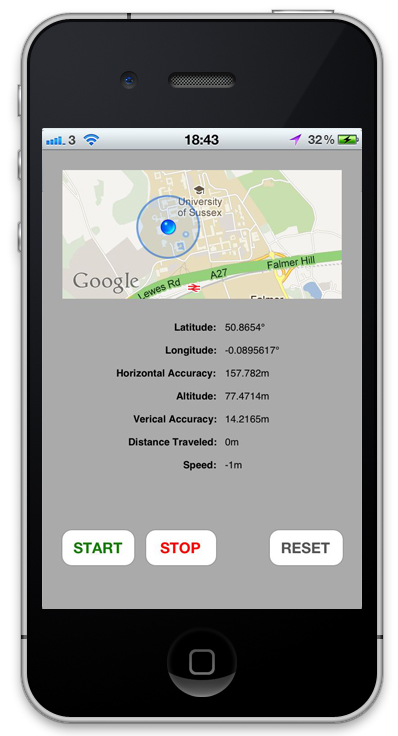
\includegraphics[width=50mm]{/content/PEM-firstPrototype.jpg}
	  \caption{The First PEM prototype}
\end{figure}


\clearpage
\section{Building a multi-view iPhone application}
From this point on in the development of the PEM the sprint cycles span through up to 4 weeks. Communication was done mostly via emails and meetings took place once a month on average. This was due to increasing complexity of implementing new features and other factors such as coping with workload from other course modules.\\ \\
The fifth sprint cycle was mostly concerned with building graphical user interface (GUI) and migrating from Xcode 3 to Xcode 4.

With a purchase of a new MacBook Pro, there was a possibility to run newest software, which was previously impossible due to old computer. Xcode 4 was a major re-write of this IDE and introduced new ways of creating iPhone applications. A feature of storyboards added to Xcode's Interface Builder (IB) enormous power as the GUI could be build from multiple views placed on a single IBs canvas resulting in more streamlined development. The Xcode migration was somewhat challenging though. Any prior knowledge of the iPhone development wasn't fully compatible with new version of Xcode and new knowledge of the same fundamentals already learned had to be acquired. This unexpectedly slowed down the development, which got back to normal when new techniques learned proved more efficient.\\ \\
As the knowledge of the iPhone development improved, in addition to MVC, concepts such as delegation and protocols had to be utilised in order to establish communication between multiple views or creating custom iPhone functionality.\\ \\
Delegation can be thought of as a design pattern. In the world of iPhone development it can be explained as follows. Apple designs some basic, standard functionality for example for how the iOS should respond to user's actions. This functionality is defined in some class e.g. UIViewController which can be thought of as a protocol. Developers of iPhone applications can make use of this protocol by declaring it in a custom class they are developing. All UIViewController functionality will now be delegated to this custom class. Developers can now use all that functionality without writing any code or build on top of it to make more sophisticated behaviour. Using a delegation is a recommended standard and is inevitable for building correct iPhone applications.\\ \\
Result of the fifth sprint cycle was a PEM prototype extended by multi view functionality. With introduction of multiple views, the application's features could be re-distributed allowing for more user-friendly design and more advanced functionality.\\ \\
Challenges faced here where how to share data between views. As previously mentioned, the PEM's functionality was directly implemented in the controller class or in other helper classes, which linked to it. This controller class was a subclass of UIViewController and therefore had to obey certain rules. A design of the iOS and the iPhone's application runtime loop for example does not allow to directly access variables in one controller from another. Further investigation had to be done to solve this problem. It turned out that there are various ways how to go about this issue. Some of them are correct and standard recommended by Apple, others are easier to understand, not recommended, but working just fine. A first approach learned to solve the issue of data exchange between controllers was using a singleton pattern. This is not Apple's standard, but is widely used and working well (more elegant way will be described later). A singleton is a class from which only one object instance can be created. This assured a single point of access. The idea was to create a singleton class (PEMDataCenter) with needed variables to share. When the controller needed to pass data to another controller, it would first store the data into PEMDataCenter. This way the data were available for use by another controllers. Following figure shows a dummy GUI with hard-coded data (at this stage only the tracking screen was connected to its controller and fully functional). There is a login screen, create profile screen, tracking screen, sessions screen, session details screen, profile screen and a sliding menu providing more options which are hidden away to prevent cluttered design. Feature such as automatic text field movement (if a form accommodates more than size of the iPhone screen) was also implemented.


\begin{figure}[H]
  \centering
	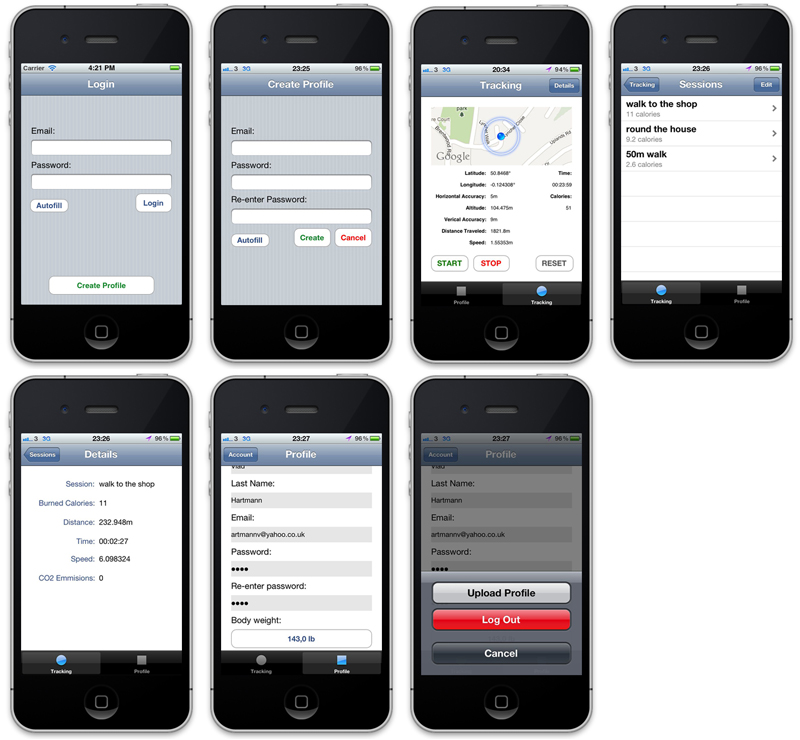
\includegraphics[width=120mm]{/content/PEM-fifthSprintCycle.jpg}
	  \caption{The PEM prototype extended by multi-view functionality}
\end{figure}


\clearpage
\section{Connecting GUI to application's logic}
In the sixth sprint cycle a main PEM's persistence mechanism and user management were implemented. PEM's requirements specifications state that the application should feature some authentication mechanism. From this point on it became apparent that PEM needed some simple database where profiles could be stored. Each profile would then have sessions (gathered and processed location data and calculations) associated with it.


\begin{figure}[H]
  \centering
	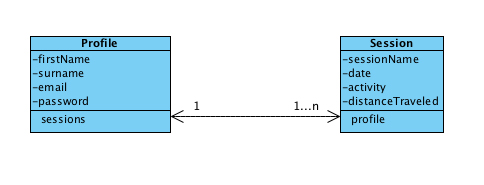
\includegraphics[width=120mm]{/content/PEM-database-Initial.jpg}
	  \caption{PEM data object diagram with relationships}
\end{figure}


This simple data model, when implemented in Xcode's data modelling tool, worked well so far. User input validation had to be in place on any text field in the GUI. This was achieved with some simple logic and regular expressions. Linking the GUI to view controllers was explained earlier in the section building a simple iPhone application. It is important to mention at this point that any additional user interface (UI) components added since the simple iPhone application had to be also wired up. Thus appropriate outlets had to be created to output data stored in view controllers' variables into these components.


\clearpage
\section{Creating a profile and logging in}
To use the PEM a user had to log in first. If the user didn't exist he/she was prompted to create a profile. The way profile creation was achieved was to create a simple profile object with attributes outlined in the PEM data object diagram above (Figure 6.9). This object then could be stored in database using Core Data persistence. Detailed procedure would consist of the following:\\ \\
Any iPhone project using a Core Data has to be configured, linking into appropriate framework and contain specific methods outlined in chosen class e.g. AppDelegate class. These methods then can be delegated to other classes as needed (so no need for a code duplication). A first step to persisting a plain object is to instantiate a Managed Object Context (MOC) by methods from the AppDelegate. A second step is to map the plain object onto Managed Object (MO). The MO is instantiated using an entity description (the data object created earlier in the Xcode's modelling tool) and from the MOC. At this stage there is a MOC containing one MO. Any values from the simple profile object can now be mapped onto the MO. To complete a data persistent procedure a save method is called on the MOC after which the data is stored in a file.\\ \\


\begin{figure}[H]
  \centering
	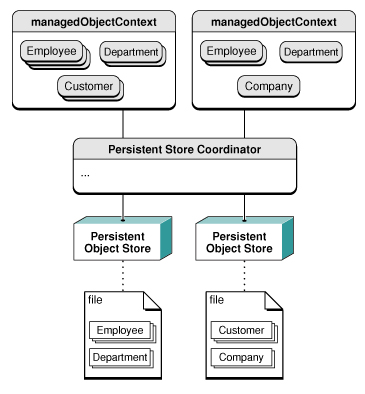
\includegraphics[width=90mm]{/content/AppleCoreData.jpg}
	  \caption{REF Apple developer website}
\end{figure}


While creating a user profile the user had to only input his/her email and two passwords that match, all in a valid formats set and verified by regular expressions. User then could add more details to his/her profile once logged in. Email address acted as a user name and therefore had to be unique. To achieve uniqueness it was necessary to query a database for any existing data. Querying in a Core Data is called fetching and is done by following procedure:\\ \\
As before a Managed Object Context (MOC) has to be instantiated. A second step is to instantiate an Entity Description (ED) object providing an object/entity that needs to be fetched and MOC. A third step is to instantiate a Fetch Request (FR) object providing the ED. A fourth step is to instantiate a Predicate (P) object providing a query and value to fetch against and set the predicate to FR. A final step is to instantiate an array by executing MOC's executeFetchRequest method with FR as a parameter and returning any results.
Once the profile was created user was prompted to login with newly created records.


\section{GPS tracking and creating a session}
Logged user was able to track his/her position and see a distance travelled. This functionality was implemented by delegating necessary object and method from a Core Location (CL) framework into the tracking view controller. The object involved was called Location Manager (LM). The method responsible for receiving and updating user's position had a basic logic, which was later extended. It was discovered that this method was being executed in a loop governed by the LM. It accepted three parameters all of which were passed in by the CL framework and iPhone GPS hardware. Any functionality inside the method could make use of these parameters. For example to calculate distance travelled a starting point was created as soon as a GPS tracking started by assigning a new location to it (only if the starting point was null). CL's method, the distanceFromLocation was called on a new location obtained passing the starting point as a parameter e.g. [newLocation distanceFromLocation: startingPoint]. The location parameters were of a type CLLocation and supported number of methods, which could be called on them to access their attributes. These attributes were for example location coordinates, horizontal or vertical accuracy or speed. For more details please refer to PEMTrackingViewController class in a source code. Any data gathered by the LM were stored in PEMLocationData object on every iteration of the method loop. This way, the PEMLocationData object contained always up-to-date values. It was used for creating a testing data sheet where values could be checked and evaluated or for sharing the values with a rest of the PEM's functionality.\\ \\
User could pause or stop GPS tracking invoking methods on the Location Manager. When stopping GPS tracking, user was asked whether to save data or not. If the user decided to save the data, a PEMsession object was created and all required data from the PEMLocationData object were stored in it (creating a separate PEMSession object rather than reusing the PEMLocationData object was necessary to separate testing and evaluating environment from ready-to-store data). The PEMSession object was then passed to a PEMDataCenter allowing sharing with other view controllers and view was switched to save session screen. Here a session name could be added and after pressing a save button the session was persisted as described in the section Creating a profile and logging in. PEMSession object now updated with a name attribute was stored back into the PEMDataCenter so a sessions view and session details view could use a newly saved data.\\ \\
This was an end of the sixth sprint cycle. PEM now was a multi view application capable of holding multiple users. It could receive and process GPS data and store it as sessions.


\clearpage
\section{Metabolic calculations}
In the seventh sprint cycle it was finally time to implement metabolic calculations, which would produce caloric expenditure. It turned out that there are various ways to do it and all depend on hardware available.\\ \\

\begin{enumerate}
	\item For example very naïve calorie expenditure estimation could be done by using calorie expenditure tables and charts. Values in the charts are estimates for a particular activity in a particular time (usually 30 min or 1h). All the PEM would need to do is to measure time of an activity user performed.\\
	\item Less naive method discovered was using walking or running equations as described in Energy Expenditure of Walking and Running, Medicine \& Science in Sport \& Exercise, Cameron et al, Dec. 2004. REF The walking equation looked like this:\\ \\

\begin{tabular}{ll}
\textbf{C = (W) x (Constant) x (D)}\\ \\
C - Calories burned\\
W - Body weight in pounds\\
Constant - 0.53 (VO2/lb/1 mile)\\
D - Distance in miles\\
\end{tabular}\\ \\


	\item Another, more precise way would be monitoring heartbeats and use them as an input into an equation. For example if the PEM had been constructed in such way that it could process signals (e.g. using iPhone headphones' microphone to listen to a heartbeats on a wrist or neck) an equation exists that can calculate the calorie expenditure REF:\\ \\


\begin{tabular}{ll}
\textbf{C = (0.6309 x H + 0.09036 x W + 0.2017 x A - 55.0969) x T / 4.184}\\ \\
C - Calories burned\\
H - Average heart rate\\
W - Body weight in pounds\\
A - Person's age\\
T - Length of exercise\\
\end{tabular}\\ \\


It has been decided however that processing the signals in the PEM would be too hard to implement in a time given.\\ \\


	\item In research by Simon Hay, Stamatina Th. Rassia , Alastair Beresford and Nick V. Baker \textsf{'}Movement dynamics in office environment' has been shown that when person accelerates, they must gain kinetic energy REF. Their energy expenditure model was expressed as:


\begin{figure}[H]
  \centering
	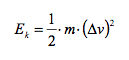
\includegraphics[width=40mm]{/content/KineticEnergy.jpg}
\end{figure}


\begin{tabular}{ll}
Ek - energy expenditure in J\\
m  - mass in kg\\
\ensuremath \Delta v - change in velocity in m/s\\
\end{tabular}\\ \\


 \item While carrying out a research of this approach it turned out that there is a relationship between the Kinetic Energy and Work REF. Therefore there is yet another way to estimate energy expenditure REF and REF:\\

\end{enumerate}

\begin{tabular}{ll}
\textbf{Wj = Fn x Dm}\\ \\
W - work in joules\\
F - force in newtons = mass x acceleration\\
D - distance in meters\\
\end{tabular}\\ \\


None of the method discovered was suitable for desired outcome of PEM and its use of GPS data. Either they have been very trivial or needed to utilize the iPhone's accelerometer hardware. While further research of available methods was under way, it has been decided to implement the Cameron's walking equation for testing purposes.

\clearpage
\subsection{ACSM MetCalcs}
Few days later a book released by American College of Sport Medicine (ACSM), the ACSM\textsf{'}s Metabolic Calculations Handbook was discovered which featured new ways of calculating caloric expenditure. Attention focused towards these ideas as they have been deemed the best solution so far.
\\ \\
The ACSM MetCalcs were introduced in 1975 in publication known as Guidelines for Exercise Testing and Prescription (GETP). It is a set of equations gathered by several authors over years from many scientific publications. The book emphasizes estimating the energy consumption by calculating values of oxygen in nonclinical environment without need for specialized and expensive hardware.

\subsubsection{Exercise science prediction}
In the exercise science prediction it is often preferred to estimate a value rather than directly measuring it. This is for various reasons such as time it takes to perform the measurement, expense of hardware involved or the inconvenience caused to the client while performing the measurement.

\subsubsection{Metabolic primer}
“Energy requirements can be expressed in terms of the oxygen requirements of the physical activity being performed – commonly referred to as the oxygen consumption or oxygen cost (VO2)” [REF]. VO2 is best known as maximal measure (VO2max) and provides useful information in area of cardiorespiratory fitness. The best possible way to measure VO2 of a physical activity is using the open-circuit spirometry. “The term open-circuit spirometry refers to the method of conducting spirometry where the subject takes a maximal inspiration from the room, inserts the mouthpiece into the mouth, and then blows out either slowly (SVC) or rapidly (FVC) until the end-of-test criterion is met” [REF]. As already mentioned, this technique is difficult to carry out in many health or fitness settings and that is why the ACSM MetCalcs became popular between health and fitness practitioners.

\subsubsection{Expression of energy use}
All actions in human body need or use energy for example for digestion of food or for muscle contraction. This is called metabolism and it is all about energy use or energy production. Energy or oxygen use can be expressed in many ways by following terms:\\
\begin{enumerate}
	\item \textbf{Metabolism} - function of time and intensity.
	\item \textbf{Exercise metabolism} - energy expenditure.
	\item \textbf{Aerobic metabolism} - production of energy using oxygen.
	\item \textbf{Oxygen consumption} - amount of oxygen (VO2) consumed typically as rate or per minute.
	\item \textbf{Relative oxygen consumption} - oxygen consumption relative to body weight, expressed in mL/kg/min.
	\item \textbf{Absolute oxygen consumption} - oxygen consumed by the person per unit of time expressed in liters per minute. It is useful because it allows for easy estimation of caloric expenditure (one liter of O2 is associated with burning of 5 kcal).
	\item \textbf{Gross VO2} - total oxygen consumption.
	\item \textbf{Net VO2} - oxygen consumption of activity only.
	\item \textbf{VO2rest} - the resting component. Value of oxygen expended at rest is estimated at 3.5 mL/kg/min.
\item \textbf{Calories} - expression of energy intake and expenditure commonly used to quantify the amount of energy derived from food. A calorie is very small unit and therefore kcal is used in calculations of human energy expenditure instead. One kcal equals 1000 calories. However conventionally it is most of the time found that terms Calories or calories are used interchangeably on packaging, which means the same as kcal. The small calorie unit is used only for scientific purposes.\\ \\
\end{enumerate}


The ACSM MetCalcs include five equations to estimate energy expenditure. The walking, running, leg ergometer (cycling), arm ergometer and stepping. With time available to implement the PEM only the walking and running equations were selected for calorie expenditure model.\\ \\

\clearpage
\subsubsection{ACSM Walking equation}
The ACSM's walking equation can be used for estimating caloric expenditure during walking activities. There are three components within the walking equation. Each of these components represents aspect of energy expenditure.

\begin{enumerate}
	\item Oxygen cost of moving one kilogram of body weight one meter. This has been estimated to be 0.1 mL/kg/m. The Horizontal Component of walking can be therefore computed as:\\

\textbf{Horizontal Component = Speed (m/min) x 0.1 mL/kg/m}\\
	
	\item To compute the Vertical Component of walking we need to know:
	\begin{enumerate}
		\item The oxygen cost of moving vertically against gravity. This has been estimated to be 1.8 mL/min/m.
		\item The rate of the movement (speed)
		\item The steepness of the vertical climb (grade)\\
	\end{enumerate}


This can be re-written as:\\

\textbf{Vertical Component = Speed (m/min) x Grade (decimal) x 1.8 mL/min/m}

\subsubsection{Computing Grade}
"Vertical ascent is denoted by grade, typically calculated as a fraction (decimal) and then converted to percent. Percent grade reflects the degree of elevation gain for give horizontal distance." [REF]\\

Example:\\

A rise of 1 m over distance of 10 m \\ =
1 m / 10 m \\ = 0.10 \\
0.10 x 100 - 10\% grade\\


	\item The Horizontal and the Vertical components represent together the net oxygen cost of walking (walking Net VO2). To obtain the gross oxygen cost of walking (walking Gross VO2) we must add in the resting component (VO2rest).
\end{enumerate}
To put it all together the ACSM walking equation is:\\ \\
\textbf{VO2 (mL/kg/min) = [Speed (m/min) x 0.1 mL/kg/m] +
          [Speed (m/min) x Grade (decimal) x 1.8 mL/min/m] +
          3.5 mL/kg/min}\\


\subsubsection{Limitations of the Walking Equation}
Results of the walking equations can only be accurate when an activity being performed is a steady-state activity. If the activity is non-steady for example the last stage of maximal exercise set, the equation will produce inaccurate results. The equation accuracy is also dependent upon a speed range between 1.9 – 3.7 miles per hour. Above the given speed range, walking economy changes and person of a particular height may run instead.\\ \\


\clearpage
\subsubsection{ACSM Running equation}
The ACSM's running equation is similar to the Walking Equation except that for running the Horizontal Component requires twice the oxygen. The Vertical Component is also different.\\ \\
The ACSM running equation is:\\ \\
\textbf{VO2 (mL/kg/min) = [Speed (m/min) x 0.2 mL/kg/m] +
          [Speed (m/min) x Grade (decimal) x 0.9 mL/min/m] +
          3.5 mL/kg/min}

\subsubsection{Limitations of the Running Equation}
As with the walking equation results of the running equation are only valid for steady-state activity. Speed must be greater than 5.0 miles per hour.\\

\clearpage
\subsubsection{Determining the oxygen cost and caloric expenditure}
We can compute caloric cost if we know the absolute VO2 in L/min.\\ \\
Example:\\ \\
Step 1. Determine the oxygen cost of walking activity.\\ \\
Speed = 2.9 miles per hour x 26.8 = 77.72 meters per minute\\
Grade = 2 \% / 100 = 0.02\\ \\
VO2 (mL/kg/min) = [77.72 (m/min) x 0.1 mL/kg/m] +
          [77.72 (m/min) x 0.02 x 1.8 mL/min/m] +
          		         3.5 mL/kg/min
		      = 7.77  + 2.80 + 3.5
		      = 14.07 mL/kg/min\\ \\
Step 2. Convert VO2 in mL/kg/min into VO2 in mL/min. We need to multiply by body weight.\\ \\
VO2 (mL/kg/min) x BW\\
= 14.07 x 65\\
= 914.55 mL/min\\ \\
Step 3. Convert VO2 in mL/min into VO2 in L/min. We need to divide by 1000.\\ \\
VO2 (mL/min) /1000\\
= 914.55 / 1000\\
= 0.91 L/min\\ \\
Step 4. Convert VO2 in L/min into kcal/min. We need to multiply VO2 (L/min) by 5.\\ \\
VO2 (L/min) x 5\\
= 0.91 x 5\\
= 4.55 kcal/min expended\\


\clearpage
\subsubsection{ACSM MetCalcs Prediction Error and Limitations}
When estimations and prediction are being made we should be willing to understand and accept some amount of error. The most common expression of prediction error is the standard error of estimate (S.E.E). Thus even though the measured VO2 at the same exercise intensity for the same individual will be very similar, it could have the S.E.E of up to 7\% for 69\% of individuals. Therefore the equations work well if tracking the same individual over time rather than comparing the VO2 between different subjects.\\ \\
As previously mentioned the equations presuppose that the activity is a steady-state one and correct equation is used in accordance with correct speed of activity.
The accuracy of equations is not affected by most environmental influences such as heat or cold but mechanical variables such as gait abnormalities, wind, snow or sand will contribute to inaccurate results.\\


\clearpage
\section{Implementing ACSM MetCalcs into PEM}
Once a knowledge ACSM's metabolic calculations has been acquired it had to be implemented into PEM. A class PEMMetabolicCalculations was created which held methods to calculate walking and running VO2 as previously explained. These methods took one parameter the PEMLocationData object containing values gathered during GPS tracking and were executed in set intervals from the PEMTrackingViewController. The values had to be converted into appropriate units. The methods returned computed VO2 values, which served as an input to calorie expenditure method.


\begin{figure}[H]
  \centering
	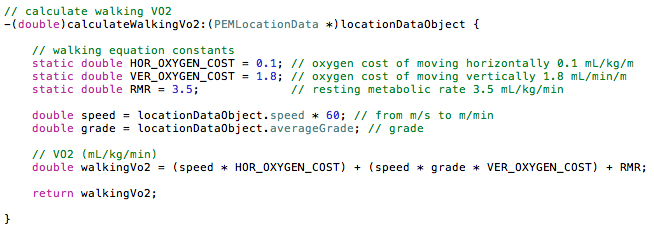
\includegraphics[width=120mm]{/content/CalculatingVO2code.jpg}
	  \caption{PEM's code snipped for calculating VO2 of walking activity}
\end{figure}


\begin{figure}[H]
  \centering
	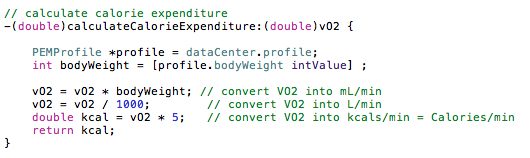
\includegraphics[width=120mm]{/content/calculatingCaloriesCode.jpg}
	  \caption{PEM's code snipped for calculating caloric expenditure}
\end{figure}

\clearpage
It is important to mention here the development stage where a grade had to be computed. 
It has been know that the grade value needed as an input to both metabolic equations can be computed by:\\
\begin{enumerate}
	\item Obtaining one position point and its altitude
	\item Travel some distance
	\item Take another position point with altitude
	\item Measure a distance between these two points
	\item Subtract the altitude of the first position point from the second one to get a rise
	\item Divide rise by distance\\
\end{enumerate}


\begin{figure}[H]
  \centering
	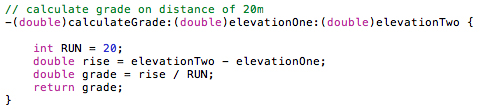
\includegraphics[width=120mm]{/content/calculateGradeCode.jpg}
	  \caption{PEM's code snipped for calculating grade}
\end{figure}


A problem however was that results of the grade computation were extremely inaccurate when using an altitude produced by iPhone's Core Location framework (as outlined in section Utilizing Apple's Core Data and Core Location). For this reason the Google Elevation API was used to obtain accurate altitude.
\\ \\
The Google Elevation API (GEAPI) is a REST web service, which provides accurate altitude data. GEAPI is free to use and devices or other software make use of it by sending a GET requests to it with latitude and longitude coordinates. Service responds with the altitude value. The response is formatted either in XML or JSON.\\ \\
The REST web service is a software system that provides functionality of some other software system, for example weather application, over the Internet. The weather application (also referred to as a server) could be written in a particular programming language like Java and therefore could be accessed over the Internet only by other Java applications called clients. A purpose of the web service is to create an intermediate point of access between the client and the weather application. The REST web service is written in such a way that clients written in various languages can communicate with it by simple commands known as HTTP verbs (GET, POST, UPDATE, DELETE). This way, if a client written in, for example, Objective-C programming language wants to know what the weather is, it sends a simple GET request to the web service, which then contacts the weather application and returns a weather data back to the client.
The XML stands for eXtensible Markup Language and it has been designed to transport and store data.


\begin{figure}[H]
  \centering
	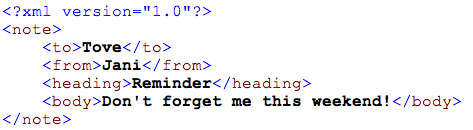
\includegraphics[width=120mm]{/content/XMLcode.jpg}
	  \caption{Example of the XML file}
\end{figure}


The JSON stands for JavaScript Object Notation and is a lightweight data-interchange format, based on the JavaScript programming language. It is easy to read and write for humans and easy for machines to generate and parse. JSON is programming language independent but uses conventions of the C-family of programming languages. JSON file is built from a collection of name/value pairs (hash table, keyed list) and an ordered list of values (array, vector, list).


\begin{figure}[H]
  \centering
	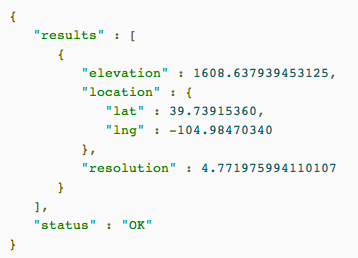
\includegraphics[width=120mm]{/content/JSONfile.jpg}
	  \caption{Example of the JSON file}
\end{figure}


To make use of the Google Elevation API web service (server) the PEM (client) had to be able to communicate with it and receive data from it. Communication had a form of sending a simple GET request to the server to which server responded by sending requested data. To send and receive data between client and server over a network following had to be done:\\

\begin{enumerate}
	\item Send data to a web service
	\begin{enumerate}
		\item Data from the client (object with variables holding the data) had to be parsed into interchangeable JSON format
		\item The interchangeable JSON data then had to be serialized (converted into array or bytes which could be carried over the network)
		\item Send data to the web service\\
	\end{enumerate}

	\item Receive data from a web service
	\begin{enumerate}
		\item De-serialize received data
		\item Map the data in JSON format onto PEM's object\\
	\end{enumerate}
\end{enumerate}

Because this procedure is very repetitive, and can introduce parsing errors the RestKit framework has been used instead.\\ \\


RestKit is an Objective-C framework for iOS that makes interacting with REST web services simple and fast. It combines a HTTP request/response API with an object mapping system. This reduces the amount of code a developers need to write so they can focus more on their data model and worry less about the details of sending requests, parsing responses, and building representations of remote resources.
An unexpected behaviour started to appear in form of a null pointer exception when attempting to receive data from GEAPI. After thorough debugging it has been found that while waiting for data to arrive from the web service, a method processing the data has been executed many times already with zero altitude. The reason for this was the asynchronous data transfer used by the RestKit framework. The asynchronous data transfer is a conventional way of sending and receiving data in a background while application is running so the GUI can remain responsive to user. By running in the background it is meant running in a separate thread of execution while GUI runs in a main thread and user can still interact with it. If the synchronous data transfer would be used, a functionality dealing with transferring data would be most likely running in the same thread as GUI, which would become frozen until data transfer is complete. A concept of asynchronous method execution is well know and there are many ways of how to deal with it. In Objective-C language, best know way is to use the notification system, also known as event handling in other programming languages, where a given method executes only if other method notifies it. The notification only takes place if some event happens, in our case, if data is received. Theory of this concept was understood but due to time constrains it could not be implemented. Instead, an iterative execution of a method that prints a word “Receiving…” was put in place to postpone further execution of code until data is received.\\ \\
With accurate altitude data received from the GEAPI and mapped onto PEMLocationData object, the PEM could use it its metabolic calculations.


\clearpage
\section{Carbon footprint calculations}
When searching for ways to calculate carbon footprint of individuals, vast majority of information sources provided ready to use CO2 emission calculators or energy conversion factor tables. The reason for this is that performing manual calculation is difficult due to huge variations in regional areas, CO2 emissions from different types of vehicles and each information source saying varying amounts. The Carbon Trust website [REF] seemed as a reliable and up-to-date source of information with estimate data of carbon footprint for individuals using a particular mode of transport.\\ \\
Implementing the CO2 emission calculations into PEM was not difficult. All that was needed was a distance and value estimate for the mode of transport from the Carbon Trust energy conversion factor table. There were three methods for calculating carbon footprint for three modes of transport the Car, Bus and Train. The following snipped of code shows the calculation for estimating CO2 emissions of PEM's user traveling by train.


\begin{figure}[H]
  \centering
	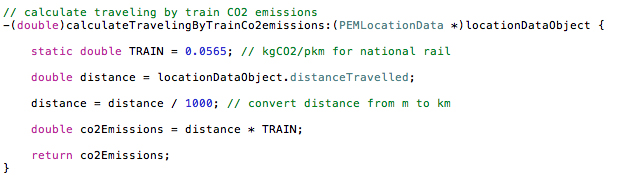
\includegraphics[width=120mm]{/content/co2CalcsTrain.jpg}
	  \caption{PEM's code snipped calculating CO2 emissions of user traveling by train}
\end{figure}


Again, as with metabolic calculations, methods to calculate CO2 emissions where invoked in intervals from the PEMTrackingViewController to give real-time data.
User of PEM even though traveling and not performing any physical activity was still expending energy and therefore notified about his/her VO2rest and caloric expenditure.\\ \\


\clearpage
\section{Implementing the PEMWEBAPP}
The aim of the eighth sprint cycle was to build a web application (PEMWEBAPP) the PEM could send a data to. This web application would store received data in its local database and present it to user once he/she would log in. At early stages of developing the PEM it was not completely decided how the web application should be built. However knowledge about building websites and utilising a network socket communication (interfaces that can plug into each other to allow programs communicate over the network) from past suggested that the PEMWEBAPP could be build.\\ \\
When development of PEM was in the final stages an introduction into course module Web Applications and Services (WAS) opened door to another solutions of how to build the PEMWEBAPP. It turned out that accessing the PEMWEBAPP's database through a socket directly from the PEM could introduce potential security risk. Utilising a knowledge obtained form WAS implementation of desired web application could begin step by step in a correct way.
One of the first steps in building a PEMWEBAPP was to set appropriate environment for web development. MySQL database, Eclipse IDE and Glassfish have been installed and configured. The Eclipse is an Interactive Development Environment where application coding is being done. The Glassfish is an open-source application server, developed by Oracle. The application server is software that provides environment for running web applications. This environment supports many features such as database connectors, web server, transaction manager, security system and many more. Database connectors are needed to create bridge between a web application and database. There is many different vendors of database systems therefore there must be connection mechanism for each of them.  Glassfish supports vast majority of connectors including a MySQL. A web server is software that serves web pages when a request arrives from a client (web browser).  A transaction manager is software that manages transactions in the application server. A transaction is a sequence of steps that must be executed to arrive at desired result. In the remote environment, for example when modifying data on Facebook profile, a sequence of steps must be performed (establish connection with database, change content of data, save data and notify user).  If at any point during execution of the steps error occurred, e.g. no Internet connection, the transaction is rolled back and data stay unchanged. The security system of an application server makes it easy to secure a web application by supporting different security realms or role managements.\\ \\
With this configuration running locally on a computer used for development (localhost) the implementation of PEMWEBAPP could start, however to test data transfer from PEM to PEMWEBAPP over a network a remote deployment environment had to be set up as well. Initial idea was to rent a remote virtual server from hosting company and perform all necessary setups as for localhost. This worked well except that cost associated with renting the server was unnecessary. After some research and with help of howtoforge.com [REF] a home server has been set up on old desktop computer. The WMware's EXSi hypervisor has been installed first. A hypervisor is a virtual machine manager used as one of many hardware virtualisation techniques. ESXi is installed directly on a physical hardware of the computer and partitions it into multiple virtual machines that can run simultaneously, sharing the physical resources of the underlying computer. Once partitioned, the Ubuntu server has been installed on one of the partitions. The Ubuntu server is a Linux server and is free. The idea of making a virtualisation was due to need to install other servers (such as windows server) in future on a single computer. One important part of this remote deployment setup was to configure home Internet router. The home server needed to be accessible from the Internet outside of house not just in local network at home. This was achieved by setting a port forwarding on a router. The port is a communication channel, which can be assigned to any program running on the computer so it can accept communication from the network. Programs such as Glassfish or MySQL database have their ports and other programs can communicate with them using these ports. Standard router setup does not provide access to any port from outside Internet for security reasons so this had to be set up in router's port forwarding table. Once set up, a request to access a particular program or resource on the home server can arrive from outside Internet to home router. From here it is channelled via a particular port to the program or resource.

\subsubsection{Java EE}
Process of developing the web application started by learning about Java Enterprise Edition (JavaEE). JavaEE is a standard set of libraries to enable programmer to write a server side code. The word standard means that the libraries are compatible with lots of application servers from different vendors such as Oracle, IBM, Red Hat, Adobe etc.

\subsubsection{Enterprise Java Beans}
Creating a java web application is very similar to creating a standard java application. The only difference is that java classes of web applications must have some additional annotation in them to be executable in the application server. By providing this annotation a basic java class becomes an Enterprise Java Bean (EJB). This EJB now has also additional features such as: its methods become transactional, secure and remote and class becomes to have easy database integration. The PEMWEBAPP has four EJB's. Two for dealing with communication from PEM and two for dealing with communication from a web browser. The IphoneDataAccessImplementation and DataAccessImplementation are both dealing with accessing PEMWEBAPP's database. They are so called Data Access Objects (DAOs). On the top of the DAOs there are the remaining two EJBs the IphoneDataManipulationImplementation and DataManipulationImplementation. These act as data manipulation classes. Because the PEMWEBAPP has nearly no business logic, these classes act only as delegates. If the application was about to be extended in future, this is the place for further functionality.


\subsubsection{Java Persistence and Entity Beans}
There are two main libraries to access database in Java. The Java Database Connectivity (JDBC) and the Java Persistence API (JPA). The JDBC is a mechanism that allows a programmer to issue SQL statements to any database that supports Java. The SQL or Structured Query Language is a programming language for managing data in relational database management systems. JDBC is suitable for some purposes but it is very low level and requires significant amount of code to be written to transfer rows of data in database into collections of java objects. On the other hand the JPA allows programmer to work with a regular java objects, and with simple annotations in classes of those objects, it will create automatically the SQL needed. Such annotated classes are called Entity Beans (EB) because they represent an entity in relational database. In a code snipped below we can see different annotations for various JPA actions such as for setting up unique, auto incrementing id of entity of setting up one-to-many relationship with any changes to be cascaded to related entity.


\subsubsection{JSF}
To write a dynamic web pages in Java (web pages that change content all the time) there are libraries such as Servlet and JSP APIs that can be used. Both are however very dated and any serious work requires tedious coding, as they are low level. Newer and more elegant solution is to use Java Server Faces (JSF), which allows a programmer to build dynamic web pages at higher level of abstraction. Instead of, for example building HTML table, JSF works using components. The components can be anything from charts, trees or buttons to image galleries.\\
To create a web page that uses JSF components we use XHTML file. XHTML stands for EXtensible HyperText Markup Language and is almost identical to HTML but it is stricter and cleaner. We need to import the JSF components library into that file by declaring an import statement at the top of the file. 
JSF is a basic components library built into JavaEE. There are many third party components libraries available and one of the most poplar and free is the PrimeFaces. PrimeFaces is an open source JSF component suite with various extensions and Ajax support. The Ajax support makes PrimeFaces very advance component library and enhances user experience. Ajax stands for asynchronous JavaScript and XML. The power of this technology is in exchanging data with a server, and updating parts of a web page, without reloading the whole page.


JSF components are well configurable to fit with web page design. Picture below shows a statistics page from the PEMWEBAPP, where a line chart component pulls caloric values from a PEMWEBAPP's database.


\begin{figure}[H]
  \centering
	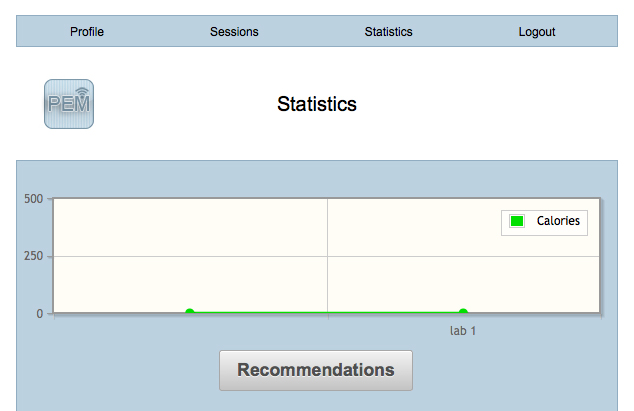
\includegraphics[width=120mm]{/content/JSFpageStats.jpg}
	  \caption{JSF page using PrimeFaces chart component displayed in a web browser}
\end{figure}


\subsubsection{Backing Bean}
Having a nice looking JSF web page is only one part of story. To make a web page dynamic we need some way of accessing a logic written in a java class. Again, as with EJB, a basic java class can be annotated to act as a Backing Bean (BB) for a web page. This backing bean will contain any required functionality and will be connected to the XHTML file created earlier. Following code snipped is from a Profile Backing Bean and shows some basic functionality that particular dynamic page needs. PEMWEBAPP has four Backing Beans, one for each page.


\subsubsection{Expression Language}
To connect the backing bean to the XHTML file we use the Expression Language (EL). EL, also known as Unified Expression Language is a special purpose programming language mostly used in Java web applications. It is used for embedding expressions into web pages. EL was developed by Java specification writers but can be used for variety of technologies. Following snipped of code shows connecting a web page to its backing bean. More specifically a line chart component accessing data from database through a Backing Bean.


\subsubsection{Dependency injection}
Many times in the web development there is a need for intercommunication between BB and EJB. To access EJB functionality in a BB we use a dependency injection. “Dependency injection is a software design pattern that allows a choice of component to be made at run-time rather than compile time.” [REF]. We can inject the Enterprise Java Bean to the Backing Bean by declaring the EJB as a variable in BB with appropriate notation. Because a database access in the PEMWEBAPP is handled by EJB we have to inject it into our Backing Bean.


\subsubsection{Creating a REST web service}
It has already been described what a REST web service is. To implement one in JavaEE we use a Java API for REST web services (JAX-RS) library and yet more annotations. The REST is built on a concept of resources. As we know the PEM will need to create or access a profile on the PEMWEBAPP. So we need to create a resource representing the profile. This is done by creating a Java class in which we describe a list of operations that we want to expose to a client, in our case the PEM. It is not important how we call these methods because client will not call them directly. The client will make a GET request with specific user id (in our case email) instead, which will be routed to a particular method annotated by the @GET annotation. We also need a URL for this method so the client will find it. Following snipped shows the required annotations to create a REST web service.\\ \\
First, a default path above the class declaration is set to represent a root. Then a specific point of access is set above appropriate method. As PEM's GET request with a specific email arrives to  method, the email is extracted from the request and used as a parameter in that method. The method then calls appropriate logic and returns results back to the client. The annotation \@Produces tells JAX-RS to parse the results into a specific format, in our case the JSON.

\subsubsection{Securing the PEMWEBAPP}
It has already been mentioned that our application server, the Glassfish, provides functionality to secure any web applications running in it. This is done by configuring application's web.xml file. The web.xml file is a configuration file that every java web application must have to be deployed onto the application server. Setting such as those for configuring a REST web service or application's security are configured here. The security of the PEMWEBAPP is set up to use user authentication with a JDBC Realm. A JDBC Realm is a way of securing a web application using a database. What this means is that user's login and password are stored in a database and encrypted. When user enters his/her credentials into a login page when logging into the PEMWEBAPP a Glassfish mechanism compares these with details stored in PEMWEBAPP's database.
We could go as far as securing the REST web service by specifying access to individual users accessing individual methods if we wanted to. In fact, the PEMWEBAPP's web service is currently open to any client with no authentication required. Data transfer between PEM and PEMWEBAPP is also not secured and data are crossing a network without being encrypted. This can cause a potential risk of data being eavesdropped or service being accessed by anyone. Both features however could not be implemented due to time constraints.


\begin{figure}[H]
  \centering
	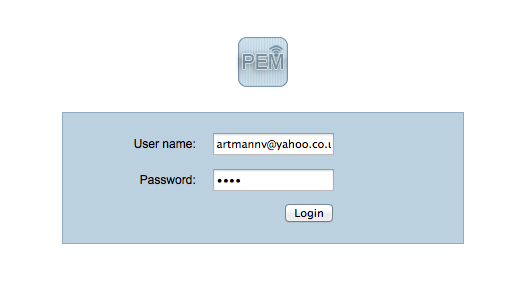
\includegraphics[width=120mm]{/content/PEMauthentication.jpg}
	  \caption{PEMWEBAPP's user authentication page}
\end{figure}



\subsubsection{Completion of PEM and PEMWEBAPP}
In the ninth sprint cycle PEM's profile upload feature was implemented as well as any final design changes to the GUI in resulting both applications being complete.\\ \\

The profile upload feature included nearly all iPhone development techniques learned so far and was considered hardest to implement. It included:\\
1.	Extensive use of RestKit and it's powerful object mapping\\
2.	Pulling data from Core Data\\
3.	Intercommunication between view controllers\\
4.	And updating GUI\\ \\

It has been briefly mentioned already that RestKit uses object mapping to send and receive data. But to really understand what is going on, here is a well-commented code snipped explaining the process:\\ \\


One of the downsides of the profile upload feature is that it does not support update. This would involve data synchronization between both PEM and PEMWEBAPP because user of the web application can delete profile online. Conceptually it is not hard to design. All that is needed is send a GET requests from PEM to PEMWEBAPP and get back a current state of user's profile. Any attempts to program this functionality however have been unsuccessful due to limited knowledge of the RestKit framework. What is happening instead is that all stored data in PEMWEBAPP's database are being replaced with those from PEM on every POST request. This way user always sees the same data in PEMWEBAPP as they are in the PEM. \\ \\

\subsubsection{Finishing the PEM's GUI}
One of the last PEM's user interface changes was to add an activity screen where user chooses the activity being monitored and recommendation popup windows. Recommendation windows are being populated with relevant content depending on a type of activity being monitored. For example if user saves a session of walking activity the recommendations will advice him/her on important facts about recommended daily caloric intake or what to do to loose or maintain weight. If user on the other hand saves a session of traveling by car, he/she will be advised about planetary wellbeing and top tips on how to reduce CO2 emissions.


\section{Maintenance and scalability}
It was difficult to pinpoint the exact stage for a solid design, however when the applications started to grow and there was a potential for scalability and maintainability further development was becoming difficult to manage. Bearing in mind possible changes to the systems in future the object-oriented design (OOD) seemed the most appropriate. Because OOD supports modularity, independent objects can be easily changed without affecting overall system. Following are the steps (as described by Ian Sommerville [REF]) used in developing both PEM and PEMWEBAPP applications. 
1.	Understanding and defining the context\\ \\


2.	Designing the system architecture
To better understand how PEM and PEMWEBAPP applications should be organised, architectural design phase has been used with focus on a design view of the applications [REF]. The design view includes architectural patterns, which are outlined below. This level of abstraction allowed both programs to be decomposed into individual components. The only correct way of developing iPhone applications is to follow a Model-View-Controller (MVC) architectural pattern, thus development of the PEM application shall be following it.\\ \\


Although the PEMWEBAPP application will be deployed on a desktop computer rather than iPhone, it has similar properties to PEM and therefore using the MVC pattern would also be a good choice. However for experimental purposes, the layered architectural pattern has been chosen instead as it is another way of achieving separation and independence.\\ \\

 
A design of the PEMWEBAPP was not as complicated as design of the PEM. And therefore the initial architecture outlined, proved to be a simple but solid application as used in enterprise environments.
 

Both, PEM and PEMWEBAPP will also comply with the Client-server architectural pattern. \\ \\


3.	Identifying the principal objects in the system
For identifying the principal objects in the system a grammatical analysis of a natural language description combined with scenario-based analysis were used. Grammatical analysis in Object-Oriented design is a technique of identifying nouns and verb. Nouns in the description refer to things (sources of classes and objects) and verbs refer to actions (sources of interactions between objects which can be though of as methods). In scenario-based analysis various scenarios of system are identified and analysed to refine object selection.\\ \\

4.	Developing design models
Following sets of class diagrams show design of most important parts of both systems. Any further development of PEM or PEMWEBAPP can be built on top of these designs.\\ \\
 



5.	Configuration management
A software project consists of several documents (files) and they all together form a configuration of the project. There is on-going need in a software development life cycle to change documents. If many people work on one particular file they may destroy one another's work. This problem can be solved by technique called version control. In essence it is version naming scheme and looks for example like this:
filename\_v0.0a.txt  - (Tom creates a text file)
filename\_v0.0b.txt  - (Eric adds some content to it)
filename\_v0.0c.txt  - (Tom replaces some content)
filename\_v0.1.txt  - (Audited by Tim and checked in)
Hannah needs to change the document and proposes the change. Proposal is accepted.
filename\_v0.1a.txt  - (Hannah check out the file)
filename\_v0.1b.txt  - (Hannah edits the file)
This process can be automated.\\ \\
Versions of both PEM and PEMWEBAPP have been managed by Git. Git is a free and open source, distributed version control system. Distributed means that each user working on a same project has a local repository. Users commit changes to their local repository. Once changes are completed they can push/pull their changes to other remote repositories. This ensures that project changes are being synchronised. As this particular project involved only one developer, myself, there was no need for synchronisation and changes were being pushed to remote GitHub repository only.
With every major change in the project a baseline was created. A baseline is reviewed and accepted version of a document, from which for all future development is derived.\\ \\



Evaluation / testing
To ensure that the PEM's metabolic calculations work as intended and produce reasonably accurate results the application had to be evaluated and calculations fine-tuned. The evaluation was done on data that were gathered and in background while application was running. Following picture shows vales produced by monitoring a walking activity. Values in the data sheet are produced by GPS tracking and by metabolic calculations.\\ \\

From the picture we can see the different elevation values being collected at two different points. These points have 20 meters distance between each other. GPS tracking method knows that it should perform a calculation of grade every 20 meters. Results of this calculation are stored in columns Grade, L Grade (Lowest Grade) and H Grade (Highest Grade). The reason for lowest and highest grade is to calculate an average grade because individual can walk uphill or downhill many times in a period of time. What we want to achieve is to have one average value of the grade in that period of time.
Values in the data sheet show estimates of caloric expenditure of myself with body weight of 63 kg. I have used 13.65 mL/kg of O2 and 4.30 kcal while walking 01.29 minute.
If compared with a table below, we can see that an individual of a similar weight (145 lbs = 65.7 kg) expends 30 kcal per 5 min, which is 6 kcal per minute.























\chapter{Conclusion}

\begin{thebibliography}{9}
  % type bibliography here
\end{thebibliography}

\chapter*{Appendices}

\end{document}






